
% load packages
\documentclass[]{article}
\usepackage{amsmath,amssymb}
\usepackage{bm}
\usepackage{lmodern}
\usepackage{xcolor}
\usepackage{hyperref}
\usepackage{url}
\usepackage{parskip}
\usepackage{graphicx}
\usepackage{subfigure}

\title{Model-based Clustering for Neural Populations}
\author{}
\date{}
\begin{document}
\maketitle

The goal for this research is to do model-based clustering for  neural populations, by making use of features for each counting process observation. 

\section{Notations}

Assume we can observe neural activities for \(N\) neurons, with counting observation up to \(T\) steps. Therefore, the observation is a \textsl{N-by-T} matrix, \(\mathbf{Y} \in \mathbb{Z}_{\geq 0}^{N \times T}\) ,with each row represents the recording from single neuron. Denote the recording for neuron \(i\) as
\(\mathbf{y}_{i} = (y_{i1},\ldots,y_{\text{iT}})'\), \(i = 1,\ldots N.\), with the cluster index for neuron \(i\) as
\(z_{i} \in \{ 1,\ldots\}\). The number of neurons in cluster \(j\) is
\(n_{j} = \sum_{i = 1}^{N}{I(z_{i} = j)}\), and
\(\sum_{j = 1,2,\ldots}^{}n_{j} = N\). The proportion/ probability in
cluster \(z_{i}\) is \(\rho_{z_{i}}\).

\section{Clustering Wrapper}
The model-based clustering problem can be transformed into fitting the mixture model (MM). The likelihood for each cluster depends on how we model the counting observation, but fitting strategies for MM are the same for all models. Here, I choose to fit the MM by Gibbs sampler. Depending on whether the number of cluster is finite or not, there are two versions: finite mixture model (FMM) and Dirichlet process mixture model (DPMM).

\subsection{Finite Mixture Model}	
Assume the number of cluster is \(J\). The full likelihood for these \(N\) neurons is
\[L = \prod_{i = 1}^{N}{\rho_{z_{i}}f\left( \mathbf{y}_{i}|\mathbf{\Theta}_{z_{i}} \right)} = \prod_{j = 1}^{J}{\rho_{j}^{n_{j}}\left\lbrack \prod_{i:z_{i} = j}^{}{f\left( \mathbf{y}_{i}|\mathbf{\Theta}_{j} \right)} \right\rbrack}\]
, where \(\mathbf{\Theta}_{j}\) contains all parameters in cluster \(j\) defined by the specific model. Therefore, the parameters need to update are:
\begin{enumerate}
	\def\labelenumi{(\arabic{enumi})}
	\item
	Cluster indicator: \(\left\{ z_{i} \right\}_{i = 1}^{N}\)
	\item
	Cluster proportion: \(\mathbf{\rho} = (\rho_{1},\ldots\rho_{J})'\)
	\item
	Model parameters: \(\mathbf{\Theta}_{j}\)
\end{enumerate}
The (conditional) priors for clustering-related parameters:
\begin{enumerate}
	\def\labelenumi{(\arabic{enumi})}
	\item
	Cluster indicator \(\left\{ z_{i} \right\}_{i = 1}^{N}\):
	\(P\left( z_{i} = j \right) = \rho_{j}\)
	\item
	Cluster proportion \(\mathbf{\rho} = (\rho_{1},\ldots\rho_{J})'\):
	\[\mathbf{\rho} \sim Dir(\delta_{1},\ldots\delta_{J})\]
	, where \(\delta_{1} = \ldots = \delta_{J} = 1\)
\end{enumerate}

So, the MCMC( Gibbs sampler) iteration for FMM is:
\begin{enumerate}
	\def\labelenumi{(\arabic{enumi})}
	\item
	Update \(\left\{ z_{i} \right\}_{i = 1}^{N}\):
	\[P\left( z_{i} = j \middle| \mathbf{y}_{i},\left\{ \mathbf{\Theta}_{j} \right\}_{j = 1}^{J} \right) \propto \rho_{j}f\left( \mathbf{y}_{i}|\mathbf{\Theta}_{j} \right)\]
	\item
	Update \(\mathbf{\rho} = \left( \rho_{1},\ldots\rho_{J} \right)^{'}\):
	\[\mathbf{\rho}|\ \left\{ \mathbf{y}_{i} \right\}_{i = 1}^{N},\ \left\{ z_{i} \right\}_{i = 1}^{N},\left\{ \mathbf{\Theta}_{j} \right\}_{j = 1}^{J} \sim Dir(\delta_{1} + n_{1},\ldots\delta_{J} + n_{J})\]
	\item
	Update \(\mathbf{\Theta}_{j}\): this is defined by the specific model. When there's no
	\(z_{i} = j\), just sample \(\mathbf{\Theta}_{j}\) from priors or by other observation-independent ways.
\end{enumerate}

\subsection{Dirichlet Process Mixture Model}

Since calculation of posterior predictive distribution can be hard or even impossible for complicated models, instead of using the popular CRP representation of DP (Neal, 2020), I choose to use the slice sampler (\href{https://www.tandfonline.com/doi/full/10.1080/03610910601096262}{Walker, 2007}).

Use the ''stick-breaking'' construction for cluster proportion, i.e.
\[\rho_{1} = \eta_{1}\]
\[\rho_{j} = \left( 1 - \eta_{1} \right) \cdot \ldots \cdot \left( 1 - \eta_{j - 1} \right)\eta_{j}\]
\[\eta_{j} \sim Beta(1,\alpha)\]

In the slice sampler for DPMM, the parameters need to update are:
\begin{enumerate}
	\def\labelenumi{(\arabic{enumi})}
	\item
	``stick-breaking'' elements: \(\eta_{j}\)
	\item
	Augment latent variable: \(\left\{ u_{i} \right\}_{i = 1}^{N}\)
	\item
	Model parameters: \(\mathbf{\Theta}_{j}\)
	\item
	Cluster indicator: \(\left\{ z_{i} \right\}_{i = 1}^{N}\)
\end{enumerate}

So, the MCMC( Gibbs sampler) iteration for DPMM is:
\begin{enumerate}
	\def\labelenumi{(\arabic{enumi})}
	\item
	update \(\eta_{j}\), for
	\(j = 1,\ldots,{{z^{*} = max}\left\{ z_{i} \right\}}_{i = 1}^{N}\) as
	\[\eta_{j}|\left\{ z_{i} \right\}_{i = 1}^{N},\ldots \sim Beta(n_{j} + 1,\ N - \sum_{l = 1}^{j}n_{l} + \alpha)\]
	\item
	update \(\left\{ u_{i} \right\}_{i = 1}^{N}\):
	\[u_{i}|\mathbf{\rho,\ldots} \sim U(0,\ \rho_{z_{i}})\]
	\item
	update \(\eta_{j}\), for \(j = z^{*} + 1,\ldots,\ s^{*}\). \(s^{*}\)
	is the smallest value, s.t.
	\(\sum_{j = 1}^{s^{*}}\rho_{j} > 1 - \min{\{ u_{1},\ldots,u_{N}\}}\)
	\[\eta_{j} \sim Beta(1,\alpha)\]
	\item
	Update \(\mathbf{\Theta}_{j}\): this is defined by the specific model. When there's no
	\(z_{i} = j\), just sample \(\mathbf{\Theta}_{j}\) from priors or by other observation-independent ways.
	\item
	Update \(\left\{ z_{i} \right\}_{i = 1}^{N}\)
	\[P\left( z_{i} = j \middle| \mathbf{y}_{i},\left\{ \mathbf{\Theta}_{j} \right\},\mathbf{\rho,}\left\{ u_{i} \right\}_{i = 1}^{N} \right) = \frac{f\left( \mathbf{y}_{i}|\mathbf{\Theta}_{j} \right)}{\sum_{j:\rho_{j} > u_{i}}^{}{f\left( \mathbf{y}_{i}|\mathbf{\Theta}_{j} \right)}}\]
\end{enumerate}

\section{linear Dynamical System Model}
Here, I model the observations by a linear dynamical system (LDS) model.

LDS models the multi-dimensional time series using a lower dimensional latent representation of the system, which evolves over time according to linear dynamics. By specifying the linear dynamics and process noise covariance, we can also handle the interactions between different neural populations (clusters).

\subsection{Model Details}
Denote the latent vector in cluster \(j\) as
\(\mathbf{x}_{t}^{(j)} \in \mathbb{R}^{p_{j}}\). For simplicity, assume all \(p_{j} = p\). Each observation follows a Poisson distribution:
\[\log\lambda_{\text{it}} = d_{i} + \mathbf{c'}_{i}\mathbf{x}_{t}^{(z_{i})}\]
\[y_{\text{it}} \sim Poisson(\lambda_{\text{it}})\]
, where \(\mathbf{c}_{i} \in \mathbb{R}^{p}\) and
\(\mathbf{x}_{t}^{(z_{i})} \in \mathbb{R}^{p}\).

Although the loading (\(d_{i}\) and \(\mathbf{c}_{i}\)) is determined by neuron index \(i\), the distribution is also cluster-dependent. That is,
\[\left( d_{i},\mathbf{c}'_{i} \right)' \sim N(\bm{\mu}_{\text{dc}}^{\left( z_{i} \right)},\mathbf{\Sigma}_{\text{dc}}^{(z_{i})})\]
By doing this, the loading within each cluster is also correlated.

Denote all latent states as \(\mathbf{x}_{t} = \left( {\mathbf{x'}_{t}^{(1)}},{\mathbf{x'}_{t}^{(2)}},\ldots \right)'\) and they evolve linearly with a Gaussian noise:
\[\mathbf{x}_{1} \sim N(\mathbf{x}_{0},\mathbf{Q}_{0})\]
\[\mathbf{x}_{t + 1}|\mathbf{x}_{t} \sim N(\mathbf{A}\mathbf{x}_{t} + \mathbf{b},\mathbf{Q})\]
For simplicity, assume \(\mathbf{Q}_{0}\) is known (e.g.
\(\mathbf{Q}_{0} = \mathbf{I} \times 10^{-2}\)).

If we assume process noise covariance is block diagonal (\href{https://papers.nips.cc/paper/2020/hash/aa1f5f73327ba40d47ebce155e785aaf-Abstract.html}{Joshua et al., 2020}), we can write things as:
\[\mathbf{x}_{t + 1}^{(j)}|\mathbf{x}_{t}^{(1)},\mathbf{x}_{t}^{(2)},\ldots \sim N(\sum_{l = 1,\ldots}^{}\mathbf{A}_{j \leftarrow l}\mathbf{x}_{t}^{(l)} + \mathbf{b}_{j},\mathbf{Q}^{(j)})\]

Notice \(\left\{ \mathbf{A}_{j \leftarrow l} \right\}\) forms the full transition matrix as:
\[\mathbf{A} = \ \begin{pmatrix}
	\mathbf{A}_{1 \leftarrow 1} & \mathbf{A}_{1 \leftarrow 2} & \ldots \\
	\mathbf{A}_{2 \leftarrow 1} & \mathbf{A}_{2 \leftarrow 2} & \ldots \\
	\ldots\  & \ldots & \ldots \\
\end{pmatrix}\]
Denote the \(j^{\text{th}}\) row block of \(\mathbf{A}\) as
\(\mathbf{A}_{j} = \begin{pmatrix}
	\mathbf{A}_{j \leftarrow 1} & \mathbf{A}_{j \leftarrow 2} & \ldots \\
\end{pmatrix}\). Then,
\(\sum_{l = 1,\ldots}^{}\mathbf{A}_{j \leftarrow l}\mathbf{x}_{t}^{(l)} + \mathbf{b}_{j}\mathbf{=}\mathbf{A}_{j}\mathbf{x}_{t} + \mathbf{b}_{j}\).

If we further let \(\mathbf{Q}\) be diagonal, with the
\(k^{\text{th}}\) row of \(\mathbf{x}_{t}\), \(\mathbf{A}\),
\(\mathbf{b}\) denoted as \(x_{\text{kt}}\), \(\mathbf{a}_{k}\), \(b_{k}\). The corresponding process noise variance is \(q_{k}\). Then:
\[x_{k,t + 1}|x_{\text{kt}} \sim N\left( \mathbf{a}_{k}^{'}\mathbf{x}_{t} + b_{k},q_{k} \right)\]

To facilitate derivation in Gibbs sampler, write the linear dynamics of
\(\mathbf{x}_{t}\) in MV-GLM form, i.e.

\[\mathbf{x}_{t + 1}^{'} = \begin{pmatrix}
	1 & \mathbf{x}_{t}^{'} \\
\end{pmatrix}\begin{pmatrix}
	\mathbf{b}^{'} \\
	\mathbf{A}^{'} \\
\end{pmatrix} + \mathbf{\epsilon}_{i}^{'}\]

, where \(\mathbf{\epsilon} \sim N(0,\mathbf{Q})\). Then if we stack the
latent by row, the problem is reduced to a multivariate general linear model (MV-GLM) problem:

\[\begin{pmatrix}
	\mathbf{x}_{2}^{'} \\
	\mathbf{x}_{3}^{'} \\
	\vdots \\
	\mathbf{x}_{T}^{'} \\
\end{pmatrix} = \begin{pmatrix}
	1 & \mathbf{x}_{1}^{'} \\
	1 & \mathbf{x}_{2}^{'} \\
	\vdots & \vdots \\
	1 & \mathbf{x}_{T - 1}^{'} \\
\end{pmatrix}\begin{pmatrix}
	\mathbf{b}^{'} \\
	\mathbf{A}^{'} \\
\end{pmatrix} + \mathbf{E}\]

, where
\(\mathbf{E} = \left( \mathbf{\epsilon}_{1},\ldots,\mathbf{\epsilon}_{T - 1} \right)^{'}\).

Since the progress noise is independent at each step,
\(f\left( \mathbf{y}_{i}|\mathbf{\Theta}_{j} \right) = \prod_{t = 1}^{T}{P(y_{\text{it}}|\mathbf{\Theta}_{j})}\),
where \(P( \cdot )\) is the Poisson density and \(\mathbf{\Theta}_{j}\) contains all parameters in cluster \(j\).

\subsection{Conditional Priors for Parameters}
The parameters need to estimate:
\begin{enumerate}
	\def\labelenumi{(\arabic{enumi})}
	\item
	Latent vectors: \(\left\{ \mathbf{x}_{t} \right\}_{t=1}^T\)
	\item
	Initials: \(\mathbf{x}_{0}\)
	\item
	Linear mapping (loading) for latent vectors:
	\(\left\{ d_{i} \right\}_{i = 1}^{N}\) and
	\(\left\{ \mathbf{c}_{i} \right\}_{i = 1}^{N}\)
	\item
	Mean and covariance for loading in each cluster:
	\(\left\{ \bm{\mu}_{\text{dc}}^{(j)} \right\}_{j}\) and
	\(\left\{ \mathbf{\Sigma}_{\text{dc}}^{(j)} \right\}_{j}\)
	\item
	Linear dynamics for latent vectors: \(\mathbf{A}\) and \(\mathbf{b}\)
	\item
	Process noise: \(\mathbf{Q}\)
\end{enumerate}

The conditional priors for these parameters:
\begin{enumerate}
	\def\labelenumi{(\arabic{enumi})}
	\item
	Latent vectors \(\left\{ \mathbf{x}_{t} \right\}_{t=1}^T\): the conditional prior is
	defined by
	\[\mathbf{x}_{1} \sim N(\mathbf{x}_{0},\mathbf{Q}_{0})\]
	\[\mathbf{x}_{t + 1}|\mathbf{x}_{t} \sim N(\mathbf{A}\mathbf{x}_{t} + \mathbf{b},\mathbf{Q})\]
	\item
	Initials \(\mathbf{x}_{0}\): assume there are \(J\) clusters,
	\[\mathbf{x}_{0} \sim N(\bm{\mu}_{\mathbf{x}_{00}},\ \mathbf{\Sigma}_{\mathbf{x}_{00}})\]
	, where \(\bm{\mu}_{\mathbf{x}_{00}} = \mathbf{0}_{\text{Jp}}\) and \(\mathbf{\Sigma}_{\mathbf{x}_{00}} = \mathbf{I}_{\text{Jp}}\)
	\item
	Linear mapping (loading) for latent vectors
	\(\left\{ d_{i} \right\}_{i = 1}^{N}\) and
	\(\left\{ \mathbf{c}_{i} \right\}_{i = 1}^{N}\):
	\[\left( d_{i},\mathbf{c}'_{i} \right)' \sim N(\bm{\mu}_{\text{dc}}^{\left( z_{i} \right)},\mathbf{\Sigma}_{\text{dc}}^{(z_{i})})\]
	\item
	Mean and covariance for loading in each cluster
	Mean and covariance for loading in each cluster
	\(\left\{ \bm{\mu}_{\text{dc}}^{(j)} \right\}_{j}\) and
	\(\left\{ \mathbf{\Sigma}_{\text{dc}}^{(j)} \right\}_{j}\):
	\[\bm{\mu}_{\text{dc}}^{(j)} \sim N(\mathbf{\delta}_{dc0},\mathbf{T}_{dc0})\]
	, where \(\bm{\delta}_{dc0} = \mathbf{0}_{p + 1}\) and
	\(\mathbf{T}_{dc0} = \mathbf{I}_{p + 1}\)
	
	\[\mathbf{\Sigma}_{\text{dc}}^{(j)} \sim W^{- 1}\left( \Psi_{dc0},\nu_{dc0} \right)\]
	, where \(\nu_{dc0} = p + 1 + 2\) and
	\(\Psi_{dc0} = \mathbf{I}_{p + 1} \times 10^{-4}\)
	
	\item
	Linear dynamics for latent vectors: \(\mathbf{A}\), \(\mathbf{b}\) and process noise \(\mathbf{Q}\).\\ 
	Denote \(\mathbf{F} = \begin{pmatrix}
		\mathbf{b}^{'} \\
		\mathbf{A}^{'} \\
	\end{pmatrix}\), \(\mathbf{f} = vec(\mathbf{F})\)
	
	\begin{align*}
		P\left( \mathbf{f},\ \mathbf{Q} \right) &= P(\mathbf{Q})P(\mathbf{f}|\mathbf{Q})\\
		\mathbf{Q} &\sim W^{- 1}(\Psi_{\mathbf{Q}_{0}},\nu_{\mathbf{Q}_{0}})\\
		\mathbf{f} &\sim N(\mathbf{f}_0, \mathbf{Q}\bigotimes \bm{\Lambda}_0^{-1})
	\end{align*}
	
	, where \(\mathbf{f}_0 = vec(\mathbf{F}_0)\).If the number of cluster is \(J\), \(\nu_{\mathbf{Q}_{0}} = Jp + 2\),
	\(\Psi_{\mathbf{Q}_{0}} = \mathbf{I}_{\text{Jp}} \times 10^{- 4}\). (To make the mean of \(\mathbf{Q}\) loosely centered around
	\(\mathbf{I}_{Jp} \times 10^{- 4}\)), \(\mathbf{F}_0 = \begin{pmatrix}
		\mathbf{0}'_{Jp} \\
		\mathbf{I}_{\text{Jp}} \\
	\end{pmatrix}\) and \(\bm{\Lambda}_0 = \mathbf{I}_{Jp + 1}\)
	
\end{enumerate}

\subsection{MCMC (Gibbs Sampler)}

\subsubsection{Update \(\left\{ \mathbf{x}_{t} \right\}_{t=1}^T\)}
Use Laplace approximation and make use of the block tri-diagonal Hessian.

Denote \(t^{\text{th}}\) column of mean firing rate and observation as \({\widetilde{\bm{\lambda}}}_{t} = \left( \lambda_{1t},\ldots,\lambda_{\text{Nt}} \right)'\)
and \({\widetilde{\mathbf{y}}}_{t} = (y_{1t},\ldots,y_{\text{Nt}})'\).
The linear mapping matrix for all observations is \(\mathbf{C}\), such that
\(\log{\widetilde{\bm{\lambda}}}_{t} = \mathbf{d} + \mathbf{C}\mathbf{x}_{t}\).
Let \(\mathbf{x} = \left( \mathbf{x'}_{1},\ldots,\mathbf{x'}_{T} \right)'\)and
\(f\left( \mathbf{x} \right) = \log{P(\mathbf{x}|\left\{ \mathbf{y}_{i} \right\}_{i = 1}^{N},\mathbf{C},\mathbf{Q}_{0},\mathbf{A},\mathbf{b},\mathbf{Q},\ldots)}\)
The first and second derivative with respect to \(\mathbf{x}\), for \(t=2, \ldots, T-1\):
\begin{align*}
	\frac{\partial f}{\partial\mathbf{x}_{1}} &= \mathbf{C'}\left( {\widetilde{\mathbf{y}}}_{1} - {\widetilde{\bm{\lambda}}}_{1} \right) - \mathbf{Q}_{0}^{- 1}\left( \mathbf{x}_{1} - \mathbf{x}_{0} \right) + \mathbf{A}'\mathbf{Q}^{- 1}\mathbf{(}\mathbf{x}_{2} - \mathbf{A}\mathbf{x}_{1} - \mathbf{b)} \\
	\frac{\partial f}{\partial\mathbf{x}_{t}} &= \mathbf{C'}\left( {\widetilde{\mathbf{y}}}_{t} - {\widetilde{\bm{\lambda}}}_{t} \right) - \mathbf{Q}^{- 1}\left( \mathbf{x}_{t} - \mathbf{A}\mathbf{x}_{t - 1} - \mathbf{b} \right) + \mathbf{A}'\mathbf{Q}^{- 1}(\mathbf{x}_{t + 1} - \mathbf{A}\mathbf{x}_{t} -\mathbf{b)}\\
	\frac{\partial f}{\partial\mathbf{x}_{T}} &= \mathbf{C'}\left( {\widetilde{\mathbf{y}}}_{T} - {\widetilde{\bm{\lambda}}}_{T} \right) - \mathbf{Q}^{- 1}\left( \mathbf{x}_{T} - \mathbf{A}\mathbf{x}_{T - 1} - \mathbf{b} \right)\\
	\frac{\partial^{2}f}{\partial\mathbf{x}_{1}\partial\mathbf{x}'_{1}} &= - \mathbf{C'}\text{Diag}\left( {\widetilde{\bm{\lambda}}}_{1} \right)\mathbf{C} - \mathbf{Q}_{0}^{- 1} - \mathbf{A}'\mathbf{Q}^{- 1}\mathbf{A}\\
	\frac{\partial^{2}f}{\partial\mathbf{x}_{t}\partial\mathbf{x}'_{t}} &= - \mathbf{C'}\text{Diag}\left( {\widetilde{\bm{\lambda}}}_{t} \right)\mathbf{C} - \mathbf{Q}^{- 1} - \mathbf{A}'\mathbf{Q}^{- 1}\mathbf{A}\\
	\frac{\partial^{2}f}{\partial\mathbf{x}_{T}\partial\mathbf{x}'_{T}} &= - \mathbf{C'}\text{Diag}\left( {\widetilde{\bm{\lambda}}}_{T} \right)\mathbf{C} - \mathbf{Q}^{- 1}\\
	\frac{\partial^{2}f}{\partial\mathbf{x}_{1}\partial\mathbf{x}'_{2}} &= \frac{\partial^{2}f}{\partial\mathbf{x}_{t}\partial\mathbf{x}'_{t + 1}} = \mathbf{A}'\mathbf{Q}^{- 1}
	&&\frac{\partial^{2}f}{\partial\mathbf{x}_{t}\partial\mathbf{x}'_{t - 1}} = \mathbf{Q}^{- 1}\mathbf{A}
\end{align*}

So, the gradient is:

\[\nabla = \frac{\partial f}{\partial\mathbf{x}} = \left( \left( \frac{\partial f}{\partial\mathbf{x}_{1}} \right)',\ \ldots,\left( \frac{\partial f}{\partial\mathbf{x}_{T}} \right)' \right)'\]

And the block tri-diagonal Hessian:

\[H = \frac{\partial^{2}f}{\partial\mathbf{x}\partial\mathbf{x}^{'}} = \begin{pmatrix}
	\frac{\partial^{2}f}{\partial\mathbf{x}_{1}\partial\mathbf{x}'_{1}} & \mathbf{A'}\mathbf{Q}^{- 1} & 0 & \cdots & 0 \\
	\mathbf{Q}^{- 1}\mathbf{A} & \frac{\partial^{2}f}{\partial\mathbf{x}_{2}\partial\mathbf{x}'_{2}} & \mathbf{A'}\mathbf{Q}^{- 1} & \cdots & \vdots \\
	0 & \mathbf{Q}^{- 1}\mathbf{A} & \frac{\partial^{2}f}{\partial\mathbf{x}_{3}\partial\mathbf{x}'_{3}} & \cdots & \vdots \\
	\vdots & \vdots & \vdots & \ddots & \vdots \\
	0 & \cdots & \cdots & \cdots & \frac{\partial^{2}f}{\partial\mathbf{x}_{T}\partial\mathbf{x}'_{T}} \\
\end{pmatrix}\]

Use Newton-Raphson to find
\(\bm{\mu}_{\mathbf{x}} =\text{argmax}_{\mathbf{x}}\left( f\left( \mathbf{x} \right) \right)\)
and \(\mathbf{\Sigma}_{\mathbf{x}}= -\left\lbrack \frac{\partial^{2}f}{\partial\mathbf{x}\partial\mathbf{x}'}\left. \ \mathbf{} \right|_{\mathbf{X} = \bm{\mu}_{\mathbf{X}}} \right\rbrack^{\mathbf{- 1}}\), such that \((P(\mathbf{x}|\left\{ \mathbf{y}_{i} \right\}_{i = 1}^{N},\ldots)\ \approx N\left(\bm{\mu}_{\mathbf{x}}, \mathbf{\Sigma}_{\mathbf{x}}\right)\).
When using Newton-Raphson (NR), \(H\backslash\nabla\) in MATLAB will make use
of block tri-diagonal structure automatically.

However, NR is not robust to bad initials. At the first few iterations, simply using fitting from previous step may lead to infinite Hessian. When the initial from previous step fails, use the approximation at recursive priors, , i.e. the adaptive smoother estimates, as the initial. The adaptive smoother estimates are from backward RTS smoother from adaptive filter, and the details about Poisson adaptive filter can be found in  \href{http://www.stat.columbia.edu/~liam/teaching/neurostat-spr11/papers/brown-et-al/eden2004.pdf}{Eden et al., 2004}.

To sample efficiently and make best use of sparse covariance, use Cholesky decomposition of
\(\mathbf{\Sigma}_{\mathbf{x}}^{- 1} = \mathbf{R}\mathbf{R}'\):
sample
\(\mathbf{Z} \sim N(\mathbf{R}'\mathbf{\mu}_{\mathbf{x}},\mathbf{I})\),
then
\(\mathbf{x} = \left( \mathbf{R}' \right)^{- 1}\mathbf{Z} \sim N(\bm{\mu}_{\mathbf{x}},\mathbf{\Sigma}_{\mathbf{x}})\).   

\subsubsection{Update \(\mathbf{x}_{0}\)}
\[P\left( \mathbf{x}_{0}|\mathbf{x}_{1},\ \mathbf{Q}_{0}\ldots \right) \propto N(\mathbf{x}_{1}|\mathbf{x}_{0},\ \mathbf{Q}_{0})N(\mathbf{x}_{0}|\bm{\mu}_{\mathbf{x}_{00}},\ \mathbf{\Sigma}_{\mathbf{x}_{00}})\]
By conjugacy, \(\mathbf{x}_{0}|\mathbf{x}_{1},\ \mathbf{Q}_{0}\ldots \sim N(\bm{\mu}_{\mathbf{x}_{0}},\ \mathbf{\Sigma}_{\mathbf{x}_{0}})\)
\begin{align*}
	\mathbf{\Sigma}_{\mathbf{x}_{0}} &= \left\lbrack \mathbf{\Sigma}_{\mathbf{x}_{00}}^{- 1} + \mathbf{Q}_{0}^{- 1} \right\rbrack^{- 1}\\
	\bm{\mu}_{\mathbf{x}_{0}} &= \mathbf{\Sigma}_{\mathbf{x}_{0}}\left( \mathbf{\Sigma}_{\mathbf{x}_{00}}^{- 1}\bm{\mu}_{\mathbf{x}_{00}} + \mathbf{Q}_{0}^{- 1}\mathbf{x}_{1} \right)
\end{align*}

\subsubsection{Update \(\left\{ d_{i} \right\}_{i = 1}^{N}\) and
	\(\left\{ \mathbf{c}_{i} \right\}_{i = 1}^{N}\)}
To update efficiently, use Laplace approximation and the error is independent for each row (i.e. update things row by row). Denote
\(\left( d_{i},\mathbf{c}'_{i} \right)' = \bm{\zeta}_{i} \in \mathbb{R}^{p + 1}\)
and \(\left( 1,{\mathbf{x}_{t}'^{\left( z_{i} \right)}} \right) = {{\widetilde{\mathbf{x}}}_{t}'^{\left( z_{i} \right)}}\).
\begin{align*}
	P\left( \bm{\zeta}_{i} \middle| \mathbf{y}_{i},\ \left\{ \mathbf{x}_{t}^{\left( z_{i} \right)} \right\}_{t = 1}^{T},\ldots \right) &= \exp{f\left( \bm{\zeta}_{i} \right)} \approx N\left( \bm{\zeta}_{i}|\bm{\mu}_{\bm{\zeta}_{i}},\mathbf{\Sigma}_{\bm{\zeta}_{i}}\  \right)\\
	\frac{\partial f}{\partial\bm{\zeta}_{i}} &= \frac{\partial l}{\partial\bm{\zeta}_{i}} - {\mathbf{\Sigma}_{\text{dc}}^{\left( z_{i} \right)}}^{- 1}\left( \bm{\zeta}_{i} - \bm{\mu}_{\text{dc}}^{(z_{i})} \right) = \left\lbrack \sum_{t = 1}^{T}{\widetilde{\mathbf{x}}}_{t}^{\left( z_{i} \right)}\left( y_{\text{it}} - \lambda_{\text{it}} \right) \right\rbrack - {\mathbf{\Sigma}_{\text{dc}}^{\left( z_{i} \right)}}^{- 1}\left( \bm{\zeta}_{i} - \bm{\mu}_{\text{dc}}^{(z_{i})} \right)\\
	\frac{\partial^{2}f}{\partial\bm{\zeta}_{i}\partial\bm{\zeta}'_{i}} &= \frac{\partial^{2}l}{\partial\bm{\zeta}_{i}\partial\bm{\zeta}'_{i}} - {\mathbf{\Sigma}_{\text{dc}}^{\left( z_{i} \right)}}^{- 1} = -\left\lbrack \sum_{t = 1}^{T}{\lambda_{\text{it}}{\widetilde{\mathbf{x}}}_{t}^{\left( z_{i} \right)}{{\widetilde{\mathbf{x}}}_{t}'^{\left( z_{i} \right)}}} \right\rbrack - {\mathbf{\Sigma}_{\text{dc}}^{\left( z_{i} \right)}}^{- 1}
\end{align*}
, where \(l\) is Poisson log-likelihood. Then use Newton-Raphson to find
\(\bm{\mu}_{\bm{\zeta}_{i}} = \text{argmax}_{\bm{\zeta}_{i}}\left( f\left( \bm{\zeta}_{i} \right) \right)\)
and \(\mathbf{\Sigma}_{\bm{\zeta}_{i}} = -\left\lbrack \frac{\partial^{2}f}{\partial\bm{\zeta}_{i}\partial\bm{\zeta}'_{i}}\left.  \right|_{\bm{\zeta}_{i} = \bm{\mu}_{\bm{\zeta}_{i}}} \right\rbrack^{-1}\). If initial as the previous step fits fails, simply use prior mean of \(\bm{\mu}_{\bm{\zeta}_{i}}\), i.e. \(\bm{\delta}_{dc0}\).

DETOUR: we can write things in the form of MV-(Poisson)-GLM as follows (in cluster j with \(n_j\) observations/ neurons, with corresponding loading be \(\mathbf{d}_{j}\) and \(\mathbf{C}_{j}\)):

\[\log\begin{pmatrix}
	\lambda_{11} & \cdots & \lambda_{1n_{j}} \\
	\vdots & \ddots & \vdots \\
	\lambda_{T1} & \cdots & \lambda_{Tn_{j}} \\
\end{pmatrix} = \begin{pmatrix}
	1 & \mathbf{x}_{1}^{'} \\
	\vdots & \vdots \\
	1 & \mathbf{x}_{T}^{'} \\
\end{pmatrix}\begin{pmatrix}
	\mathbf{d}_{j}^{'} \\
	\mathbf{C}_{j}^{'} \\
\end{pmatrix} + \mathbf{E}_j\]

We can further organize things column-wise. let \(\begin{pmatrix}
	1 & \mathbf{x}_{1}^{'} \\
	\vdots & \vdots \\
	1 & \mathbf{x}_{T}^{'} \\
\end{pmatrix} = \mathbf{G}\), then the design matrix and corresponding log-mean response are \(\begin{pmatrix}
\mathbf{G} & \mathbf{0} & \cdots & \mathbf{0} \\
\mathbf{0} & \mathbf{G} & \cdots & \mathbf{0} \\
\vdots & \vdots & \ddots & \vdots \\
\mathbf{0} & \cdots & \cdots & \mathbf{G} \\
\end{pmatrix}\) and \({\log\begin{pmatrix}
	\lambda_{11}^{(j)} & \cdots & \lambda_{T1}^{(j)} & \lambda_{12}^{(j)} & \cdots & \lambda_{T2}^{(j)} & \cdots & \lambda_{Tn_{j}}^{(j)} \\
\end{pmatrix}}'\).

However, when I use the Laplace approximation and NR, because of the block-diagonal structure of design matrix, the error is always independent observation by observation. This is equivalent to observation-wise update as above.

\textbf{Maybe I did something wrong?}
The point to say this is to make loading within each cluster depends on each other. Check these two later(\href{https://www.tandfonline.com/doi/full/10.1080/03610926.2012.743565?journalCode=lsta20}{ref1} and \href{https://www.tandfonline.com/doi/full/10.1080/02664763.2021.1877637?src=recsys}{ref2}).

Now I do it in another way: make the prior cluster-dependent...

\subsubsection{Update \(\left\{ \mathbf{\mu}_{\text{dc}}^{(j)} \right\}_{j}\) and \(\left\{ \mathbf{\Sigma}_{\text{dc}}^{(j)} \right\}_{j}\)} \label{loading prior}

Purpose: to make loading within each cluster depends on each other, and this will help with clustering. As above, denote \(\left( d_{i},\mathbf{c}'_{i} \right)' = \bm{\zeta}_{i} \in \mathbb{R}^{p + 1}\).
\begin{enumerate}
	\def\labelenumi{(\arabic{enumi})}
	\item
	Mean \(\left\{ \bm{\mu}_{\text{dc}}^{(j)} \right\}_{j}\): by
	conjugacy, \(\bm{\mu}_{\text{dc}}^{(j)} \sim N\left( \bm{\delta}_{\text{dc}},\mathbf{T}_{\text{dc}}\  \right)\)
	\begin{align*}
		\mathbf{T}_{\text{dc}}^{- 1} &= \left( \mathbf{T}_{dc0}^{- 1} + n_{j}{\mathbf{\Sigma}_{\text{dc}}^{(j)}}^{- 1} \right)^{- 1}\\
		\bm{\delta}_{\text{dc}} &= \mathbf{T}_{\text{dc}}\left( \mathbf{T}_{dc0}^{- 1}\bm{\delta}_{dc0} + {\mathbf{\Sigma}_{\text{dc}}^{(j)}}^{- 1}\sum_{i:z_{i} = j}^{}\bm{\zeta}_{i} \right)
	\end{align*}
	\item
	Covariance \(\left\{ \mathbf{\Sigma}_{\text{dc}}^{(j)} \right\}_{j}\): by conjugacy, \(\mathbf{\Sigma}_{\text{dc}}^{(j)} \sim W^{- 1}\left( \Psi_{\text{dc}},\nu_{\text{dc}} \right)\)
	\begin{align*}
		\nu_{\text{dc}} &= n_{j} + \nu_{dc0}\\
		\Psi_{\text{dc}} &= \Psi_{dc0} + \sum_{i:z_{i} = j}^{}{\left( \bm{\zeta}_{i} - \bm{\mu}_{\text{dc}}^{(j)} \right)\left( \bm{\zeta}_{i} - \bm{\mu}_{\text{dc}}^{(j)} \right)'}
	\end{align*}
\end{enumerate}

\subsubsection{Update \(\mathbf{A}\), \(\mathbf{b}\) and \(\mathbf{Q}\)} 
Here, I only give the update for full \(\mathbf{Q}\). If we want to assume block-diagonal or diagonal structure of \(\mathbf{Q}\), just update things cluster-by-cluster or latent-by-latent.

As shown before, the problem is the usual Bayesian MV-GLM problem. Denote \(\mathbf{F} = \begin{pmatrix}
	\mathbf{b}^{'} \\
	\mathbf{A}^{'} \\
\end{pmatrix}\), \(\mathbf{f} = vec(\mathbf{F})\), \(\mathbf{Y}_\mathbf{bA} = (\mathbf{x}_{2}, \mathbf{x}_{3} \ldots, \mathbf{x}_{T})'\) and \(\mathbf{X}_\mathbf{bA} = \begin{pmatrix}
1 & \mathbf{x}_{1}^{'} \\
1 & \mathbf{x}_{2}^{'} \\
\vdots & \vdots \\
1 & \mathbf{x}_{T - 1}^{'} \\
\end{pmatrix}\)

\[\mathbf{Y}_\mathbf{bA} = \mathbf{X}_\mathbf{bA}\mathbf{F}+ \mathbf{E}\]

, where
\(\mathbf{E} = \left( \mathbf{\epsilon}_{1},\ldots,\mathbf{\epsilon}_{T - 1} \right)^{'}\) and \(\mathbf{\epsilon} \sim N(0,\mathbf{Q})\). Then posteriors are
\begin{align*}
	\mathbf{Q}|\mathbf{Y}_{\mathbf{\text{bA}}},\mathbf{X}_{\mathbf{\text{bA}}},\ldots &\sim W^{-1}(\Psi_{\mathbf{Q}}, \nu_{\mathbf{Q}})\\
	\mathbf{f}|\mathbf{Y}_{\mathbf{\text{bA}}},\mathbf{X}_{\mathbf{\text{bA}}},\mathbf{Q},\ldots &\sim N(vec(\mathbf{F}_\mathbf{bA}),  \mathbf{Q}\bigotimes \bm{\Lambda}_\mathbf{bA}^{-1})
\end{align*}
, with parameters be:
\begin{align*}
	\Psi_{\mathbf{Q}} &= \Psi_{\mathbf{Q}_{0}} + (\mathbf{Y}_\mathbf{bA} - \mathbf{X}_\mathbf{bA}\mathbf{F}_\mathbf{bA})'(\mathbf{Y}_\mathbf{bA} - \mathbf{X}_\mathbf{bA}\mathbf{F}_\mathbf{bA}) + (\mathbf{F}_\mathbf{bA} - \mathbf{F}_0)'\bm{\Lambda}_0(\mathbf{F}_\mathbf{bA} - \mathbf{F}_0)\\
	\nu_{\mathbf{Q}} &= \nu_{\mathbf{Q}_{0}} + T - 1\\
	\mathbf{F}_\mathbf{bA} &= (\mathbf{X}'_\mathbf{bA}\mathbf{X}_\mathbf{bA} + \bm{\Lambda}_0)^{-1}(\mathbf{X}'_\mathbf{bA}\mathbf{Y}_\mathbf{bA} + \bm{\Lambda}_0\mathbf{F}_0)\\
	\bm{\Lambda}_\mathbf{bA} &= \mathbf{X}'_\mathbf{bA}\mathbf{X}_\mathbf{bA} + \bm{\Lambda}_0
\end{align*}


\section{Model Check [Problems for \(\mathbf{b}\) and \(\mathbf{A}\) partially solved]} \label{problems}

\subsection{Estimation of \(\mathbf{d}\) and \(\mathbf{C}\) alone}
First, turn off all others except for loading (related) parameters and set them to be true values. There are 2 versions: (1) update priors as in subsection \ref{loading prior} and (2) no update of priors, and just set the prior for each as the standard normal.
For the estimation with prior update, the results are mean from iteration 50 to 100 (Figure \ref{loading alone}).
\begin{figure}[h!]
	\makebox[\linewidth][c]{%
		\centering
		\subfigure[]{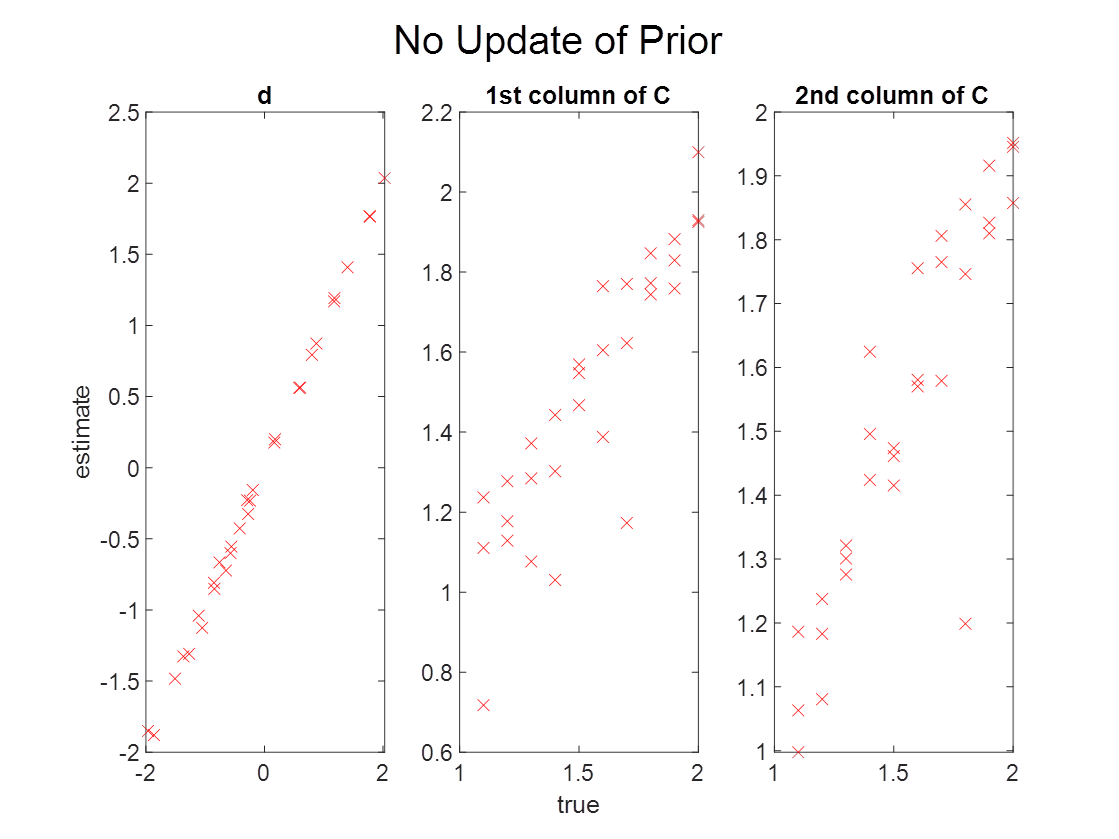
\includegraphics[width=0.6\textwidth]{image016.png}}%
		\subfigure[]{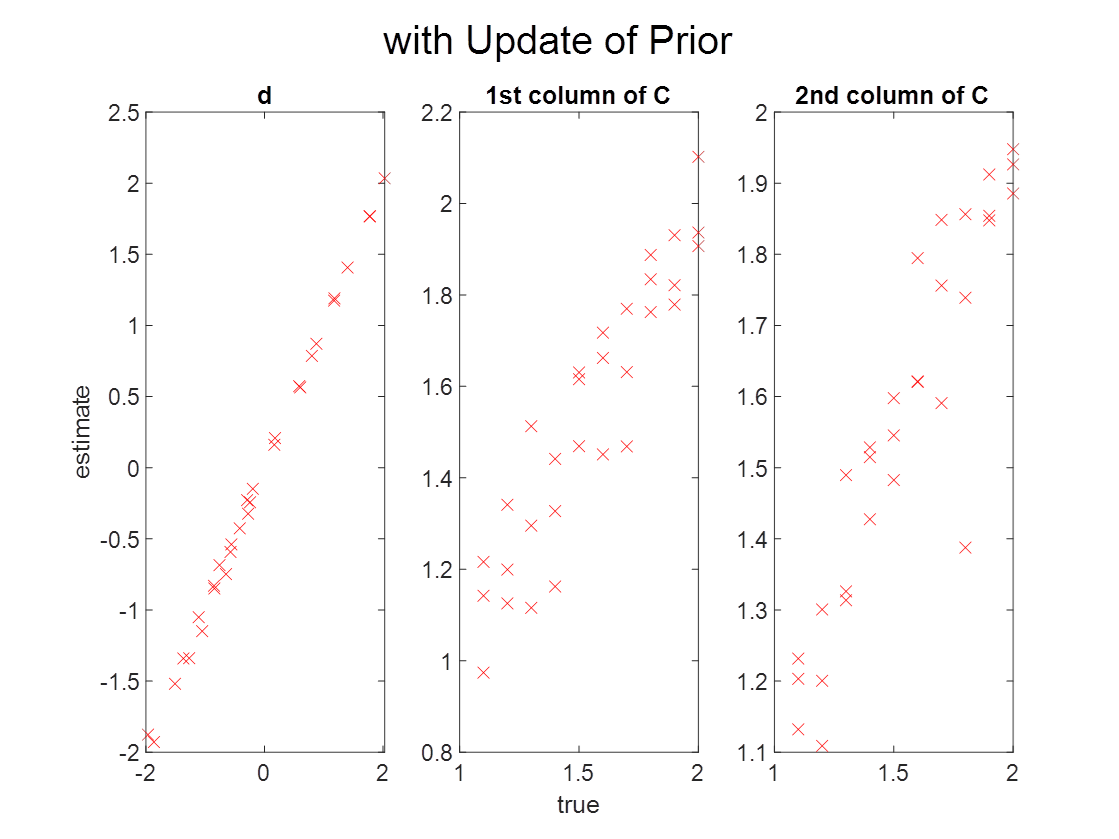
\includegraphics[width=0.6\textwidth]{image017.png}}%
	}
	\caption{estimation of loading}
	\label{loading alone}
\end{figure}

The mixing of convergence for loading priors (in subsection \ref{loading prior}) are fine. The update of priors don't influence results a lot, but this will help clustering a lot. It seems estimation of loading is fine. Let's see what happens when estimation of latents \(\mathbf{x}_t\) is on at the same time.

\subsection{Estimation of \(\mathbf{d}\), \(\mathbf{C}\) and \(\mathbf{x}_{t}\)}
When the estimation of \(\mathbf{x}_t\) is on, we need more iterations. The results are mean from iteration 500 to 1000 (Figure \ref{loading and latent}).

The estimation of loading:
\begin{figure}[h!]
	\makebox[\linewidth][c]{%
		\centering
		\subfigure[]{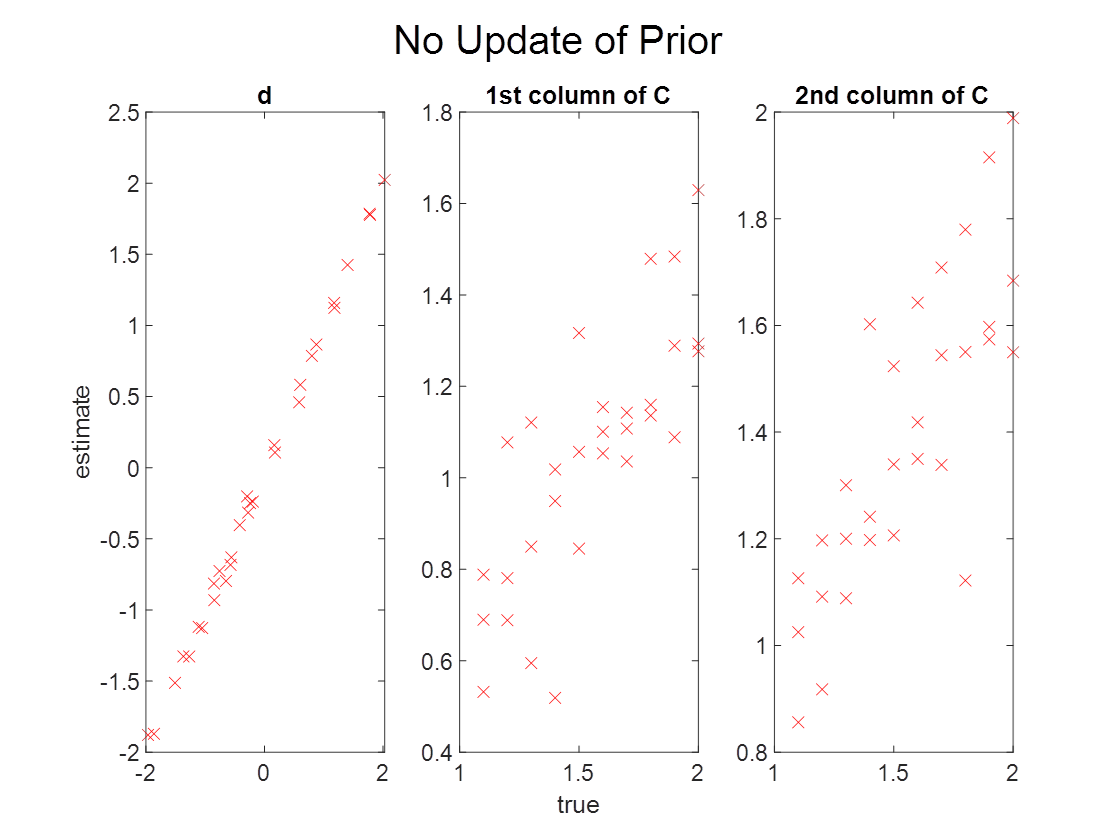
\includegraphics[width=0.6\textwidth]{image018.png}}%
		\subfigure[]{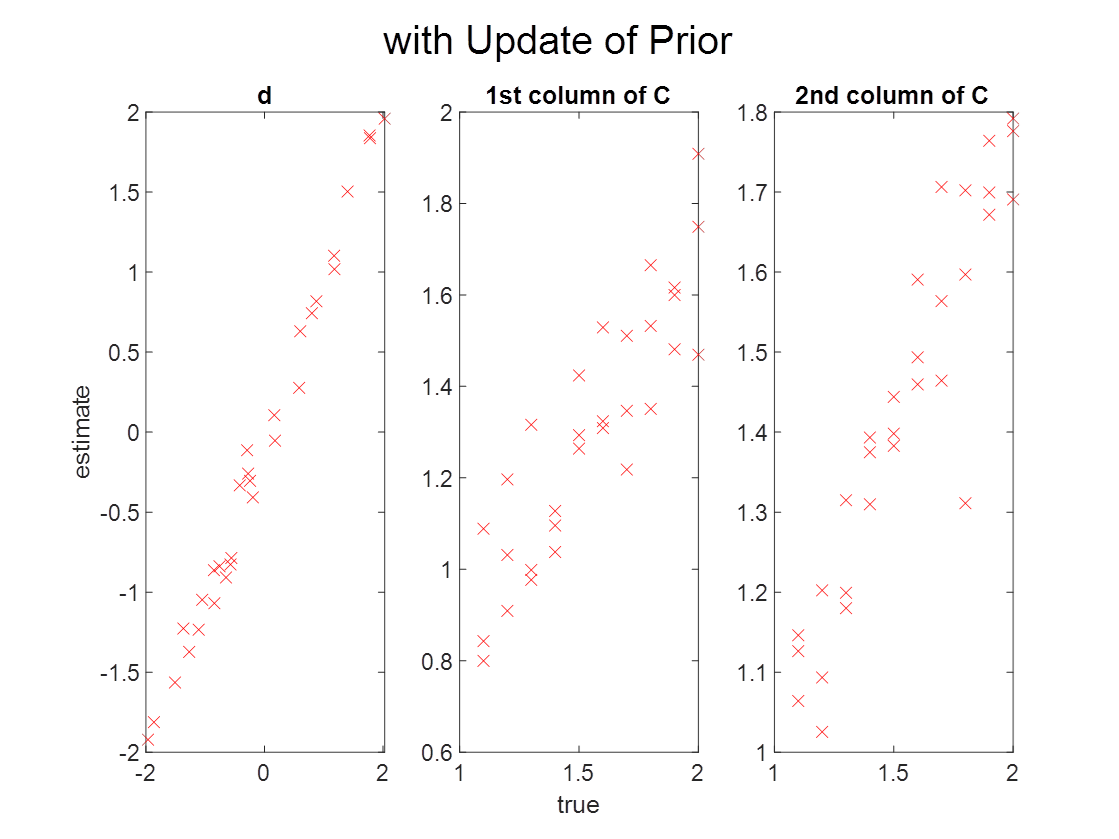
\includegraphics[width=0.6\textwidth]{image020.png}}%
	}
	\caption{estimation of loading, with latents on}
	\label{loading and latent}
\end{figure}

And the estimation of corresponding latents (Figure \ref{loading and latents}):
\begin{figure}[h!]
	\makebox[\linewidth][c]{%
		\centering
		\subfigure[no update of prior]{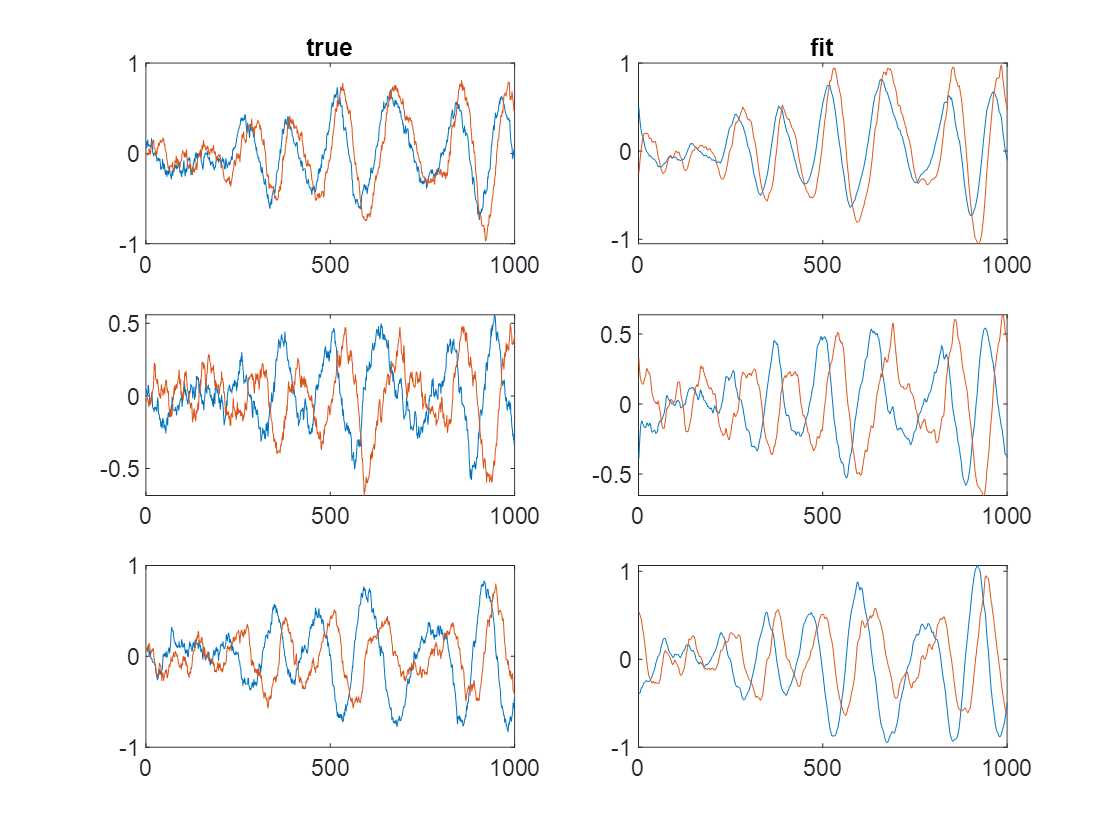
\includegraphics[width=0.6\textwidth]{image019.png}}%
		\subfigure[with update of prior]{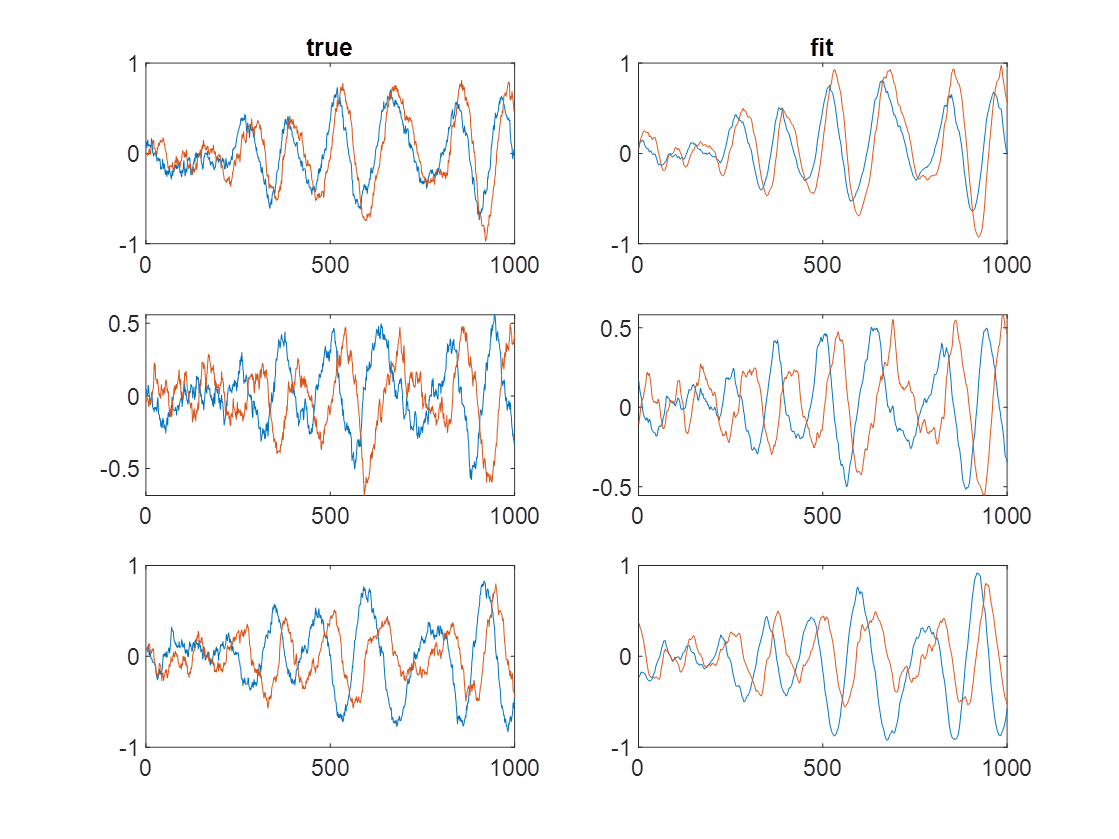
\includegraphics[width=0.6\textwidth]{image021.png}}%
	}
	\caption{estimation of loading}
	\label{loading and latents}
\end{figure}

Things are still fine. The remaining parts may influence latent estimations are dynamics (\(\mathbf{b}\), \(\mathbf{A}\)) and prior process noise \(\mathbf{Q}\).

\subsection{Estimation of \(\mathbf{b}\), \(\mathbf{A}\), \(\mathbf{Q}\) and \(\mathbf{x}_t\)}
I show the results of block-diagonal (Figure \ref{bAQX_blkDiag}) and full (Figure \ref{bAQX_full}) \(\mathbf{Q}\). These results are from 2000 MCMC samples. The latent and dynamics are from average from 500 to 2000 iterations.

\begin{figure}[h!]
	\makebox[\linewidth][c]{%
		\centering
		\subfigure[trace]{\label{fig:a}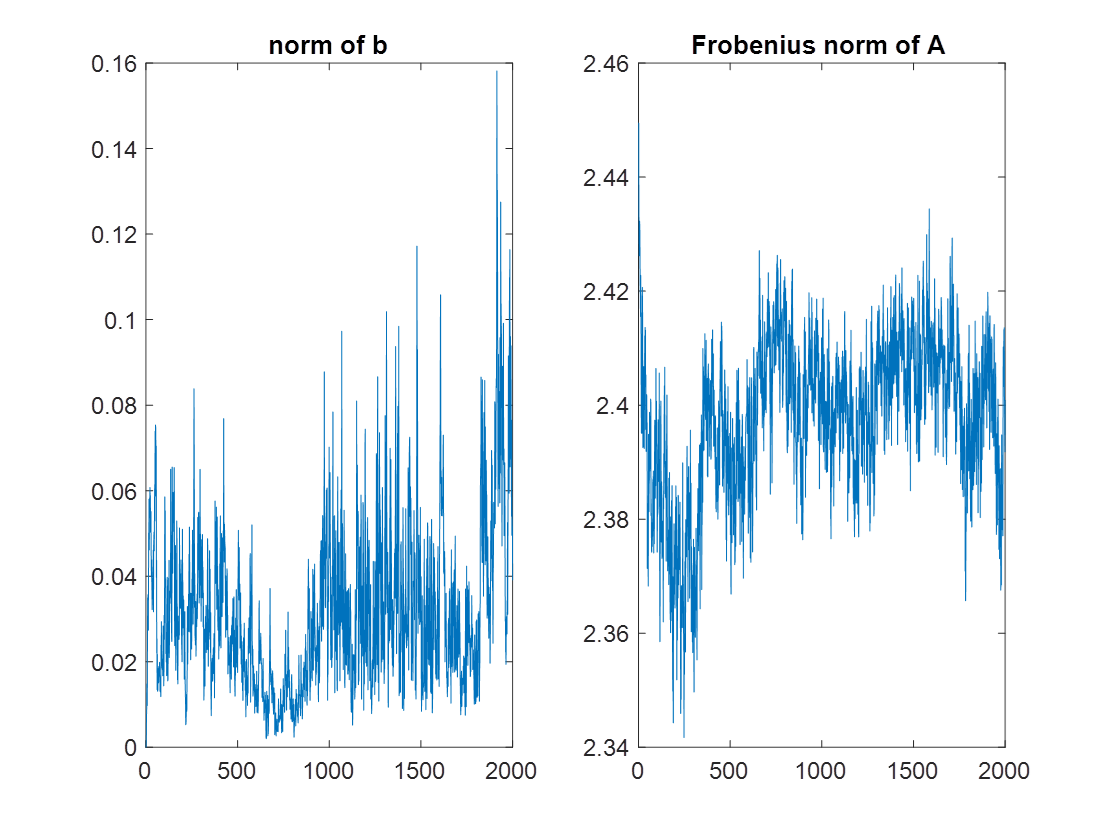
\includegraphics[width=0.55\textwidth]{bAX_blkDiag_trace.png}}%
		\subfigure[latent]{\label{fig:b}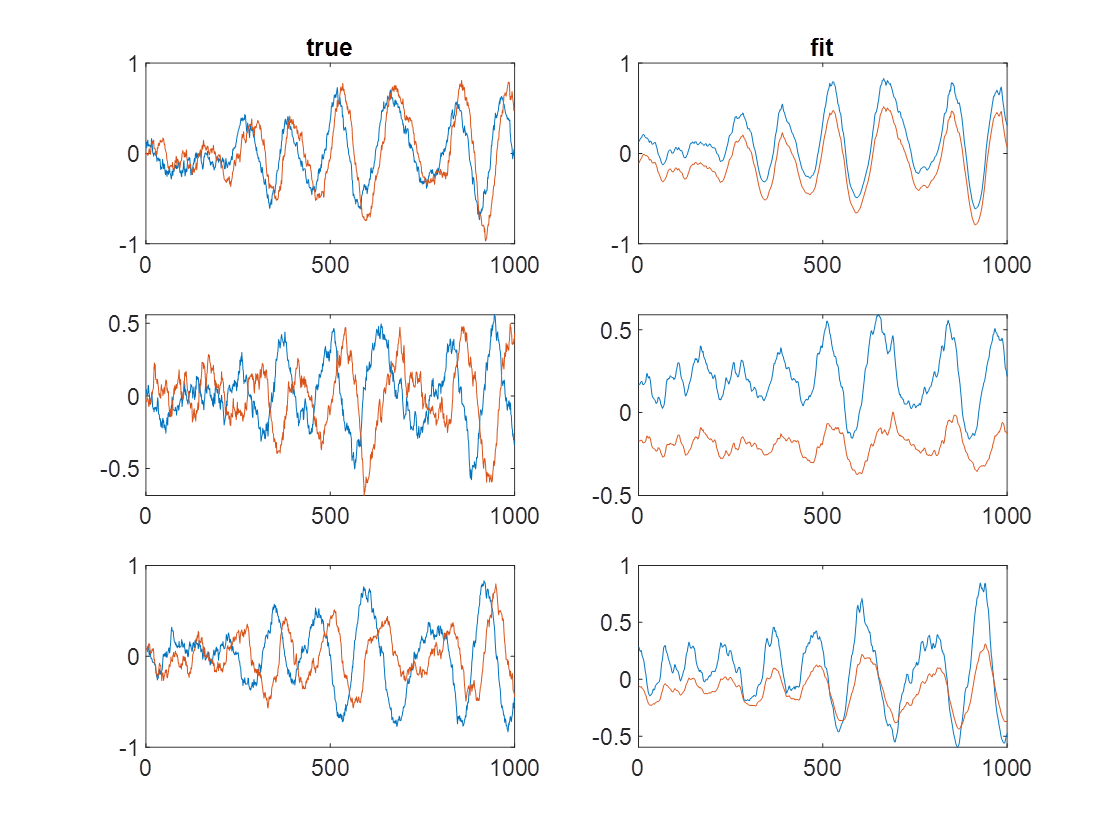
\includegraphics[width=0.55\textwidth]{bAX_blkDiag_latent.png}}%
		\subfigure[dynamics \(\mathbf{A}\)]{\label{fig:c}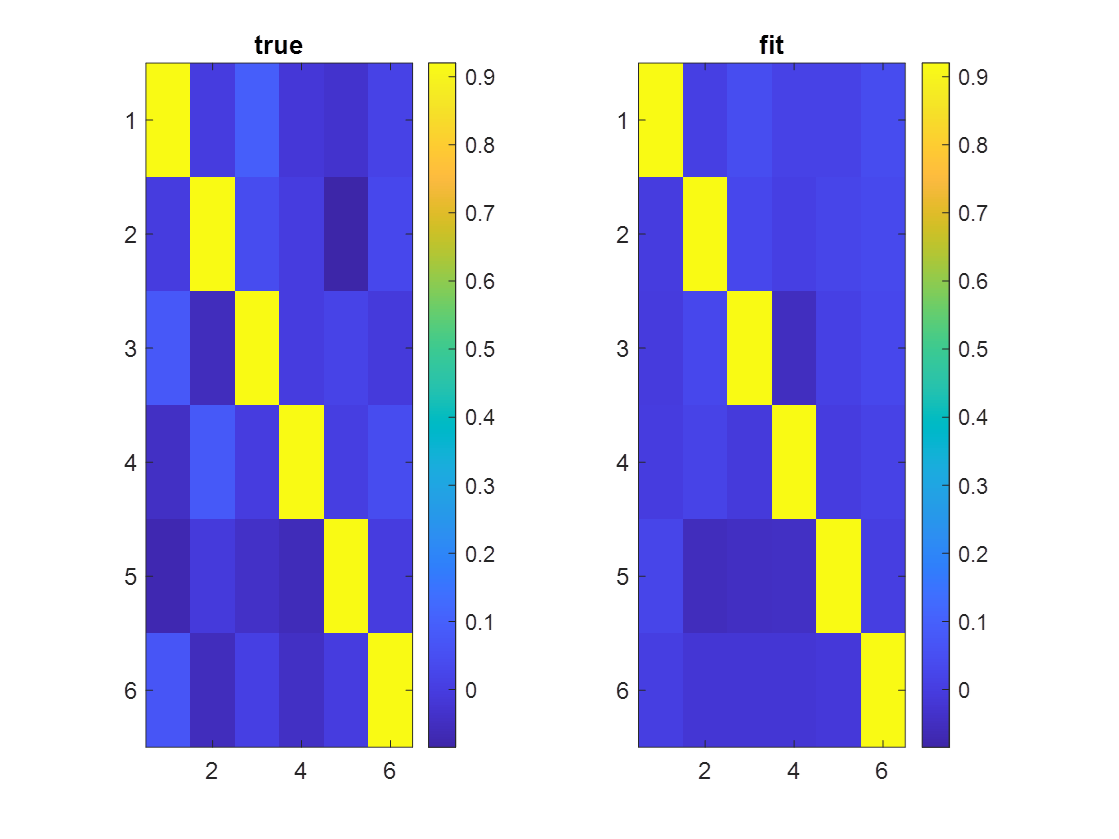
\includegraphics[width=0.55\textwidth]{bAX_blkDiag_A.png}}%
	}
	\caption{sampling of $\mathbf{b}$, $\mathbf{A}$, $\mathbf{Q}$ and $\mathbf{x}_t$, block-diagonal process noise}
	\label{bAQX_blkDiag}
\end{figure}

\begin{figure}[h!]
	\makebox[\linewidth][c]{%
		\centering
		\subfigure[trace]{\label{fig:a}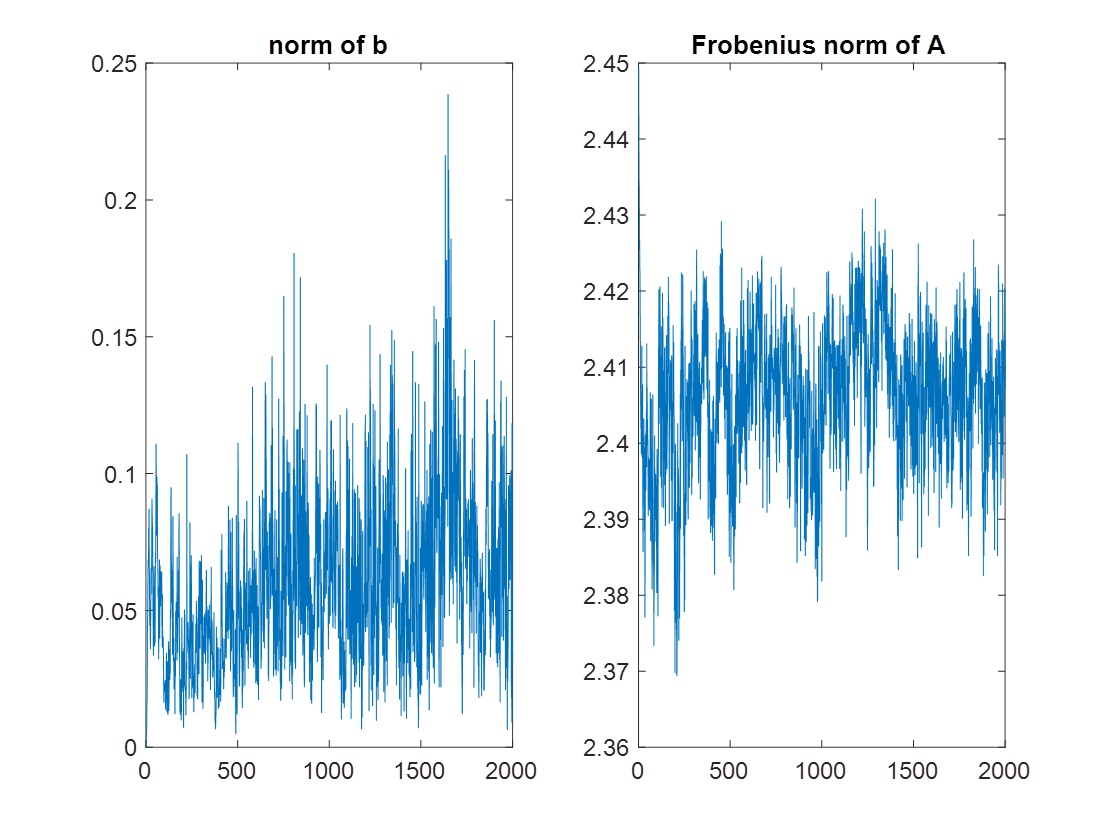
\includegraphics[width=0.55\textwidth]{bAX_full_trace.png}}%
		\subfigure[latent]{\label{fig:b}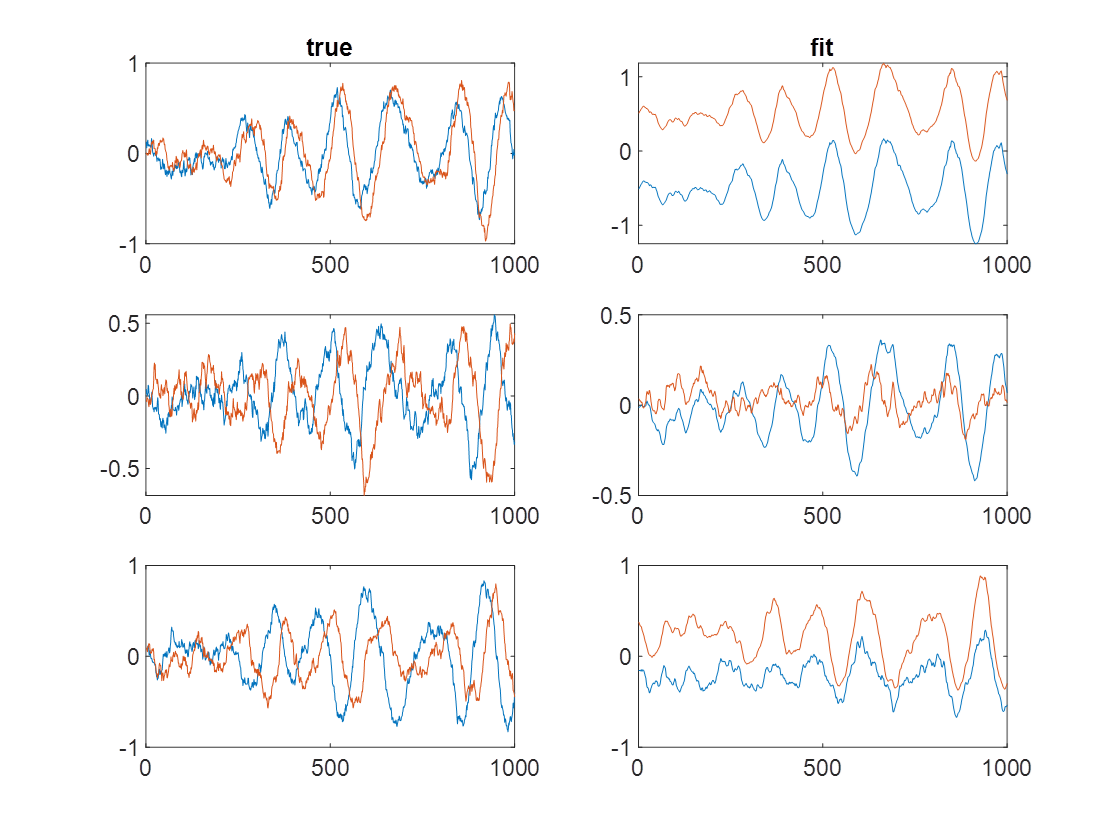
\includegraphics[width=0.55\textwidth]{bAX_full_latent.png}}%
		\subfigure[dynamics \(\mathbf{A}\)]{\label{fig:c}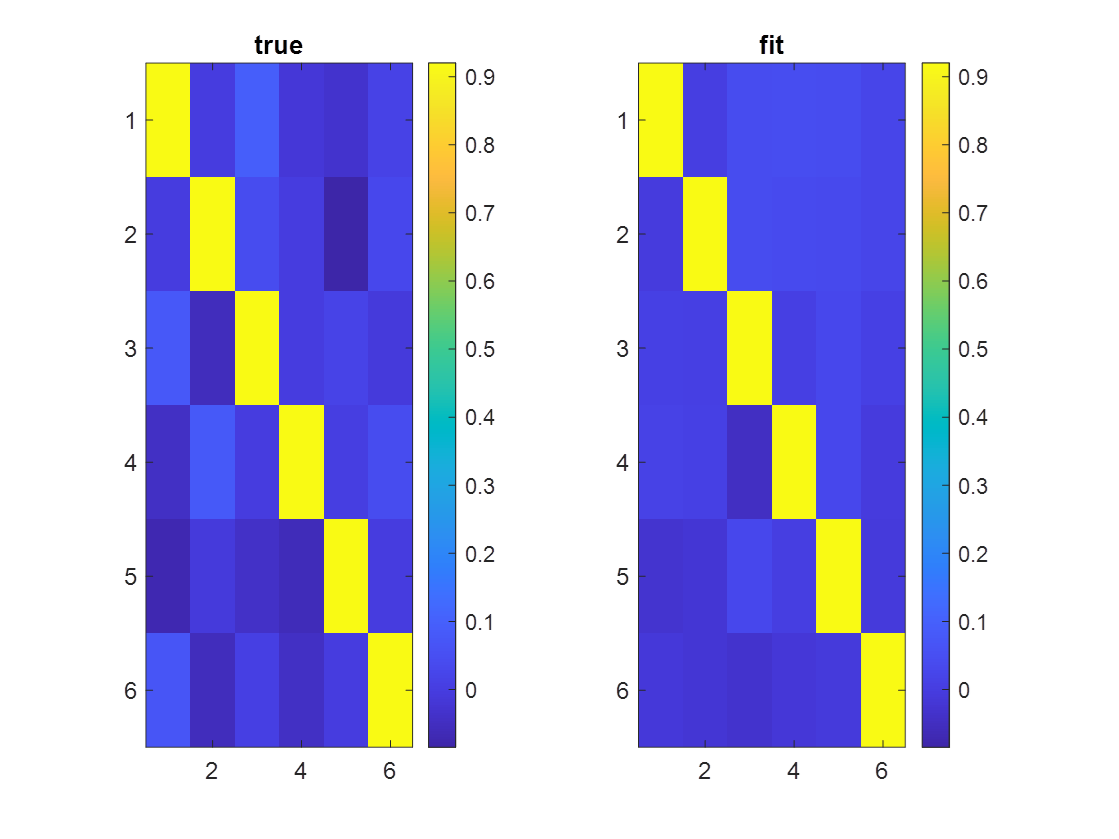
\includegraphics[width=0.55\textwidth]{bAX_full_A.png}}%
	}
	\caption{sampling of $\mathbf{b}$, $\mathbf{A}$, $\mathbf{Q}$ and $\mathbf{x}_t$, full process noise}
	\label{bAQX_full}
\end{figure}

Both block-diagonal and full looks fine, but the mixing of  full process noise version looks better.


\section{Simulations}

There are two set of simulation examples. The first example is generated from LDS model directly, while in the second example the latents are generated directly without explicit specifying linear dynamics. In all following results, I fit things with both \href{https://github.com/weigcdsb/state-space-clustering/tree/main/LDS/blkDiag}{block-diagonal} and \href{https://github.com/weigcdsb/state-space-clustering/tree/main/LDS/full}{full} \(\mathbf{Q}\). The fitting results for block-diagonal version is a bit better, because the underlying true \(\mathbf{Q}\) is diagonal. In the following part, I only show results from block-diagonal fitting for labeled data. For unlabeled data, i.e. clustering, all the results can be found in this \href{https://github.com/weigcdsb/state-space-clustering/tree/main/results/gif}{folder}.

\subsection{Simulation 1: Generate from LDS Directly}
In this simulation, there are 3 clusters with 10 neurons in each cluster. The dimension of latents in each cluster is 2. In the linear dynamics, the bias term \(\mathbf{b}\) is zero. There's no within-population interaction but has some weak between-population interactions. In other words, the linear dynamics matrix \(\mathbf{A}\) is roughly diagonal. The details of simulation can be found in the first section of the \href{https://github.com/weigcdsb/state-space-clustering/blob/main/LDS/blkDiag/lds_sample_DP_blkDiag.m}{simulation 1}.

\subsubsection{Labeled Data: No Clustering}
The code for fitting is \href{https://github.com/weigcdsb/state-space-clustering/blob/main/LDS/blkDiag/lds_sample_DP_blkDiag.m}{here}. After running 2000 iterations, the trace of the sample is shown in Figure \ref{lds norms}.
\begin{figure}[h!]
	\centering
	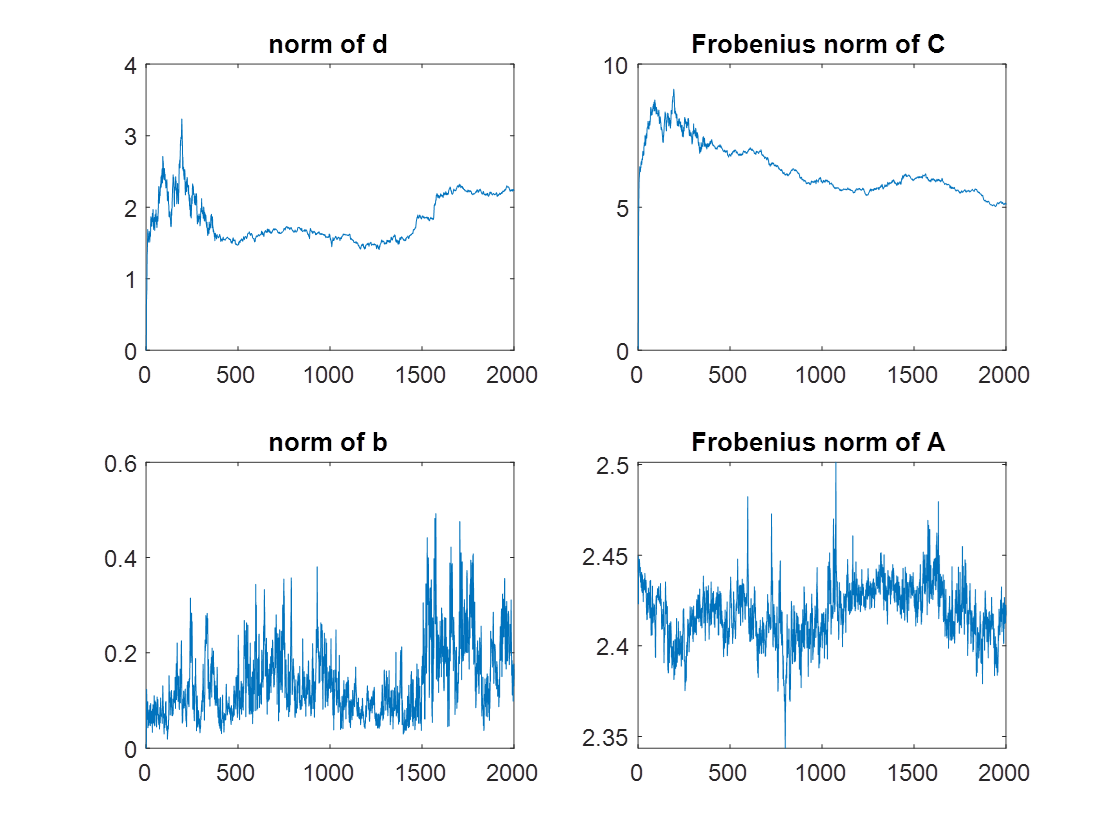
\includegraphics[width = .8\textwidth]{lds_blk_trace.png}
	\caption{(Frobenius) norm for \(\mathbf{d}\), \(\mathbf{C}\), \(\mathbf{b}\) and \(\mathbf{A}\)}
	\label{lds norms}
\end{figure}\\

Some results are in Figure \ref{fig:LDS labeled}. These are means from iteration 1000 to 2000.

\begin{figure}[h!]
	\makebox[\linewidth][c]{%
		\centering
		\subfigure[overall mean firing rate]{\label{fig:a}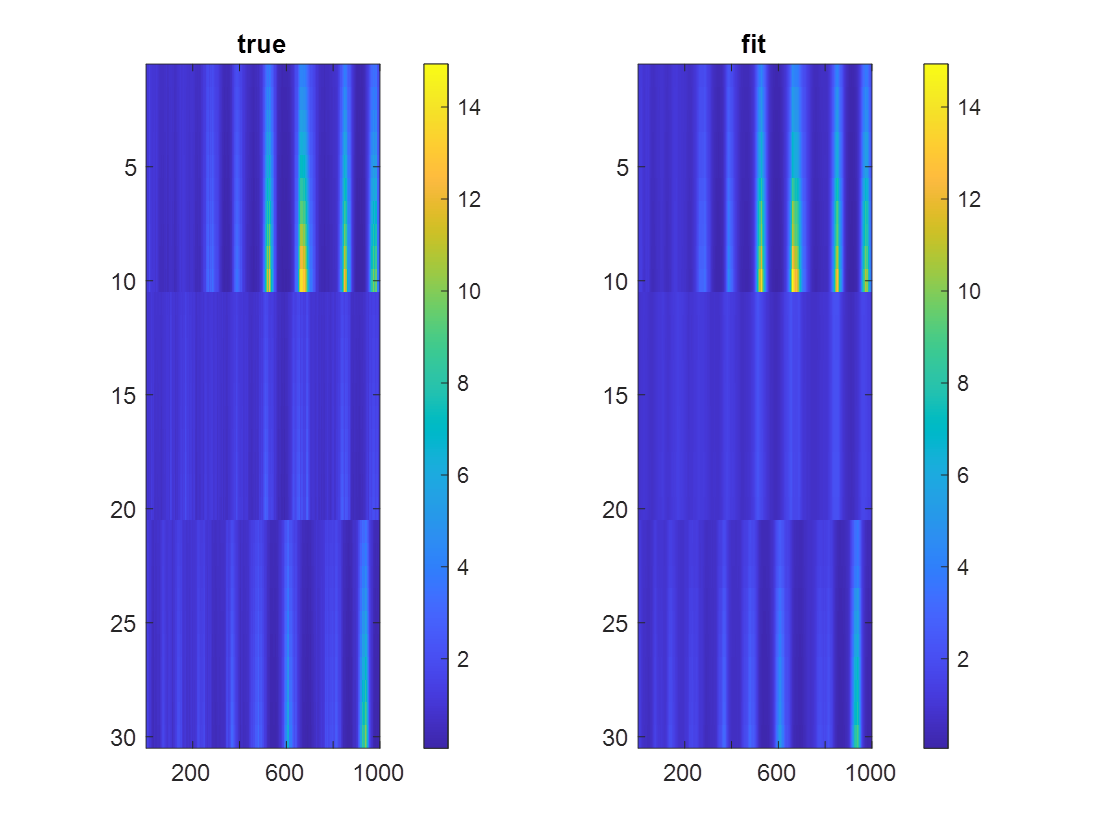
\includegraphics[width=0.55\textwidth]{lds_blk_FR.png}}%
		\subfigure[latents]{\label{fig:b}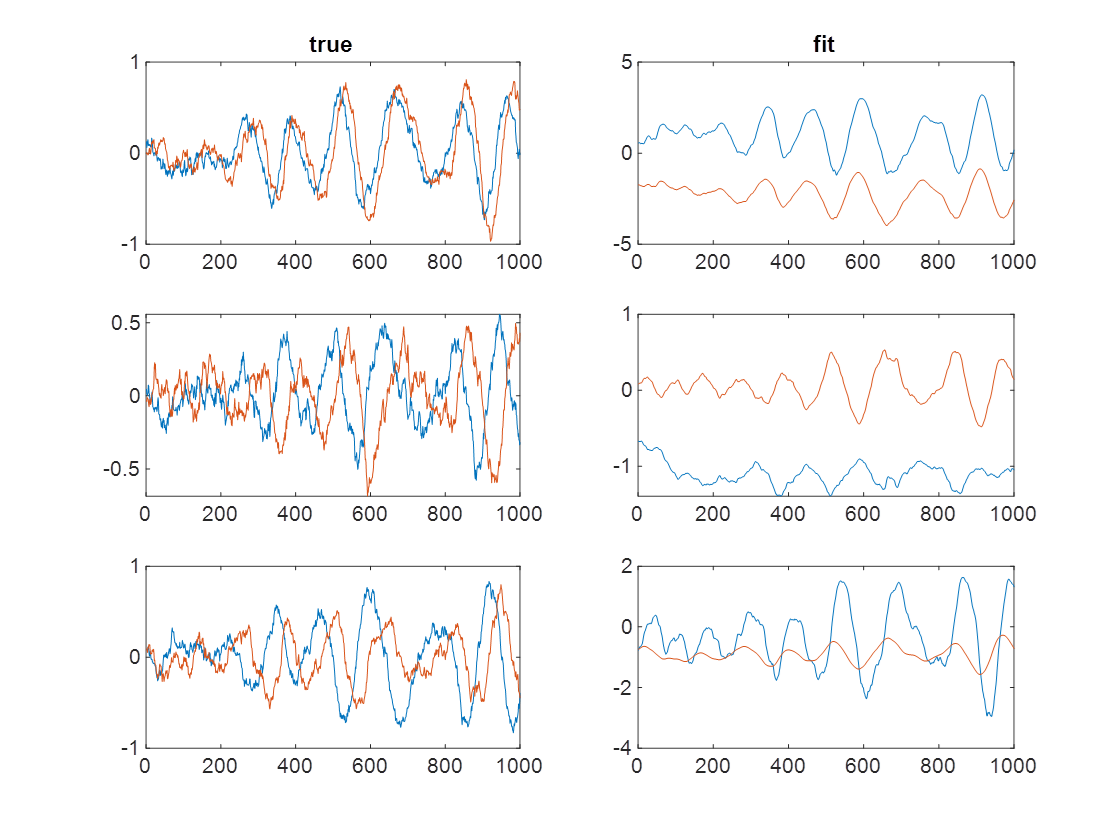
\includegraphics[width=0.55\textwidth]{lds_blk_latent.png}}%
		\subfigure[dynamics \(\mathbf{A}\)]{\label{fig:c}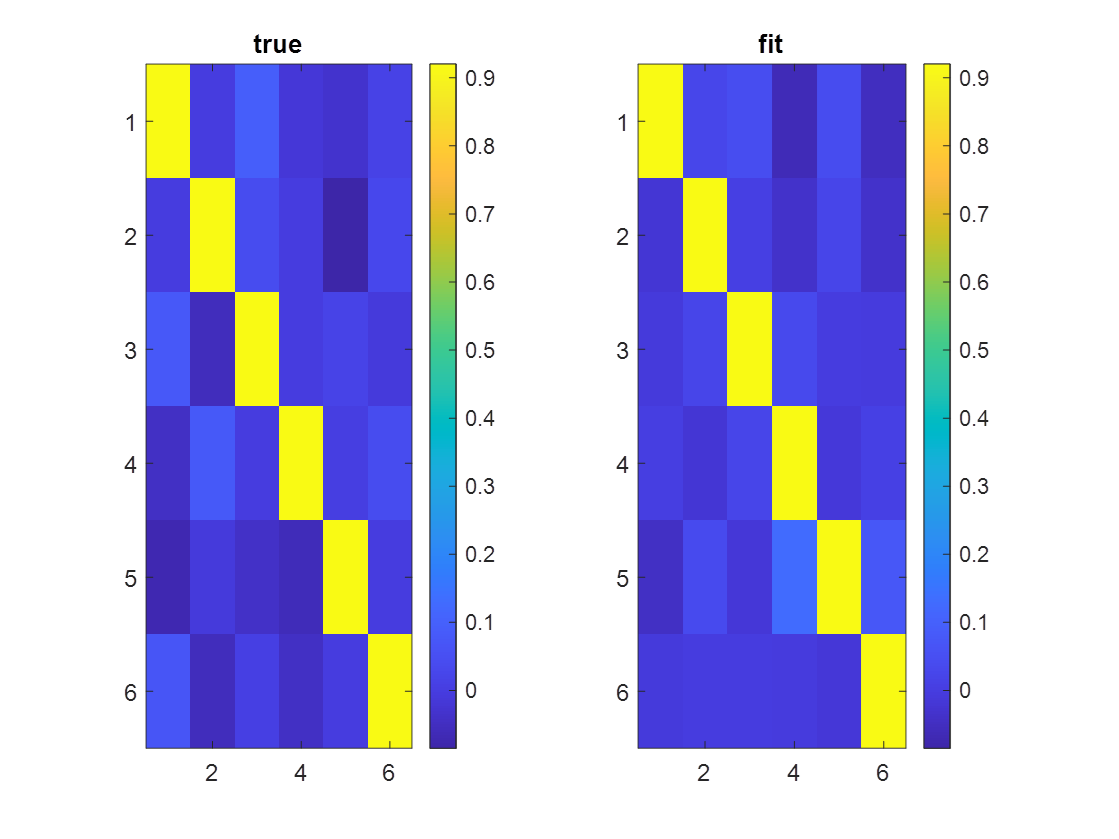
\includegraphics[width=0.55\textwidth]{lds_blk_A.png}}%
	}
	\caption{LDS sample with labels}
	\label{fig:LDS labeled}
\end{figure}

Personally, I think the fitting is not bad and the mixing is fine (in previous version, we may need 10000 iterations to get a not bad result. But here 2000 iterations did even better than before).

I also fit the model by assuming one cluster. Again, the fitting for overall mean firing rate is perfect. This is why it's important to make the loading, \(\mathbf{d}\) and \(\mathbf{C}\), also be cluster-dependent (loading within clusters are correlated).

If the loading only depends on neuron index and will not change for different clustering assignments, it's impossible to do clustering (at least in this case), since the loading is enough to capture all the patterns.

\textbf{Think more on it.} Maybe we can do MV-(Poisson)-GLM, to make all loading within cluster correlated.


\subsubsection{Unlabeled Data: Clustering}
To give the full path of clustering, I show results in GIFs. All results can be found in this \href{https://github.com/weigcdsb/state-space-clustering/tree/main/results/gif}{folder}. The code can be found in this \href{https://github.com/weigcdsb/state-space-clustering/tree/main/LDS/blkDiag}{folder}.

Basically, in my current implementation, algorithms are good to merge clusters. However, generating new clusters is very hard... In other words, the newly generated cluster will usually not be sampled.

\textbf{This is a big problem}. This makes DPMM loses its power. \textbf{Fix that later}.

\subsection{Simulation 2: Generate Latents, without Specifying Linear Dynamics}
In this simulation, there are again 3 clusters with 2 latents and 10 neurons in each. Now, the latents are generated directly without specifying the underlying linear dynamics of latents. However, each latent is generated independently, so the linear dynamics matrix \(\mathbf{A}\) should be roughly diagonal. The details of simulation can be found in the \href{https://github.com/weigcdsb/state-space-clustering/blob/main/LDS/blkDiag/unspecifiedA_sample_blkDiag.m}{code}.

\subsubsection{Labeled Data: No Clustering}
As in simulation 1, the data is fitted by the true cluster assignment (3 clusters) and forcing all neurons belong to single cluster. The code can be found \href{https://github.com/weigcdsb/state-space-clustering/blob/main/LDS/blkDiag/unspecifiedA_sample_blkDiag.m}{here}.

This time I ran 1000 iterations. The trace of the samples is shown in Figure \ref{noA norms}.
\begin{figure}[h!]
	\centering
	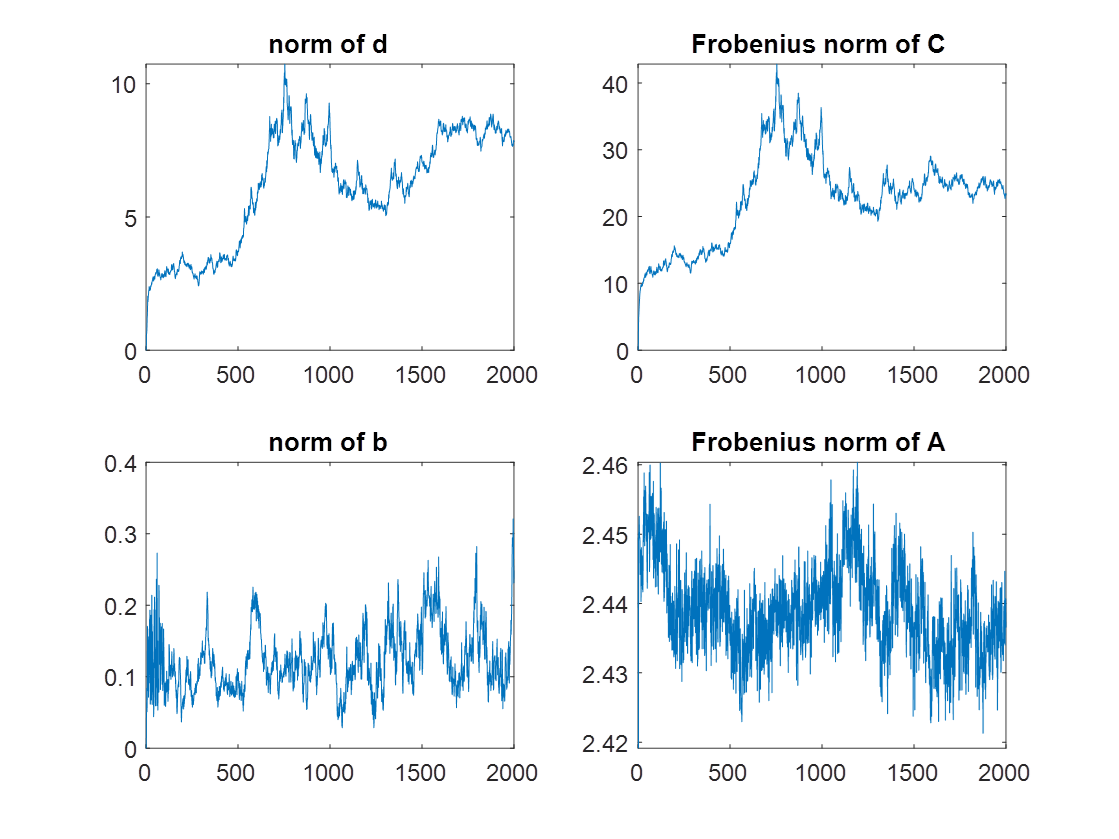
\includegraphics[width = .8\textwidth]{noA_blk_trace.png}
	\caption{(Frobenius) norm for \(\mathbf{d}\), \(\mathbf{C}\), \(\mathbf{b}\) and \(\mathbf{A}\)}
	\label{noA norms}
\end{figure}\\

Some results are in Figure \ref{fig:noA labeled}. These are means from iteration 500 to 1000.

\begin{figure}[h!]
	\makebox[\linewidth][c]{%
		\centering
		\subfigure[overall mean firing rate]{\label{fig:a}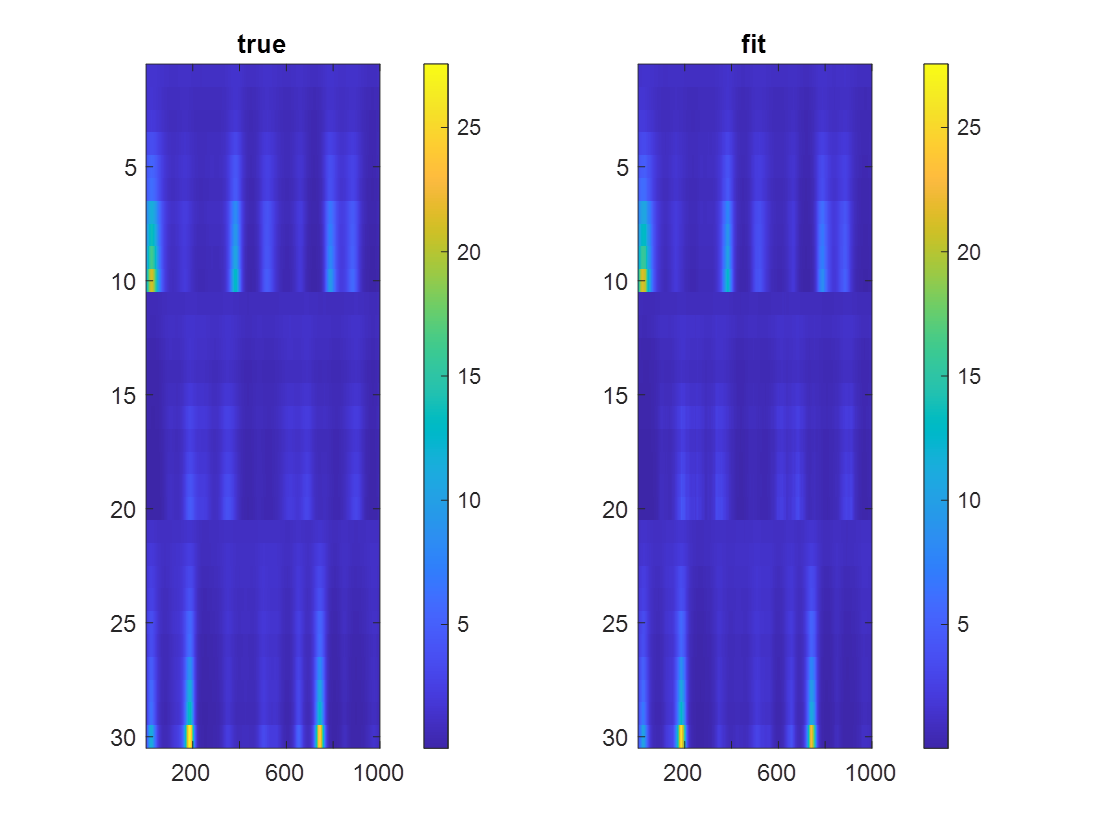
\includegraphics[width=0.55\textwidth]{noA_blk_FR.png}}%
		\subfigure[latents]{\label{fig:b}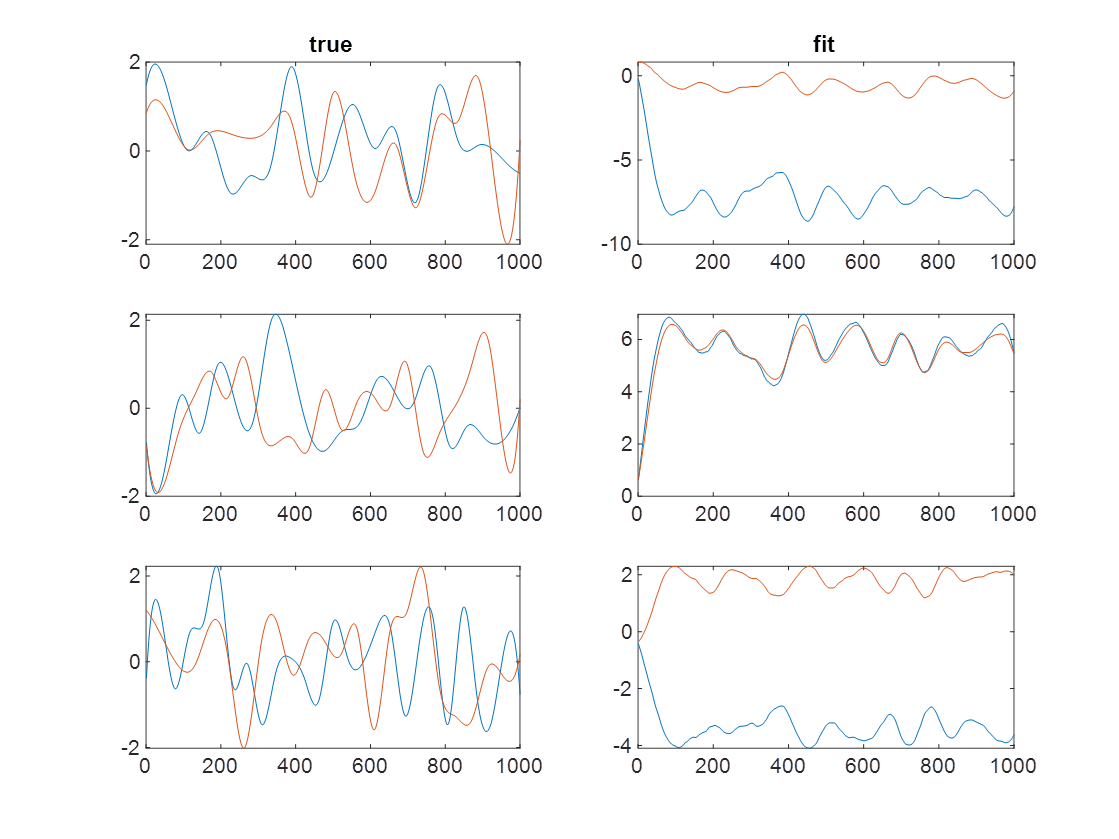
\includegraphics[width=0.55\textwidth]{noA_blk_latent.png}}%
		\subfigure[dynamics \(\mathbf{A}\)]{\label{fig:c}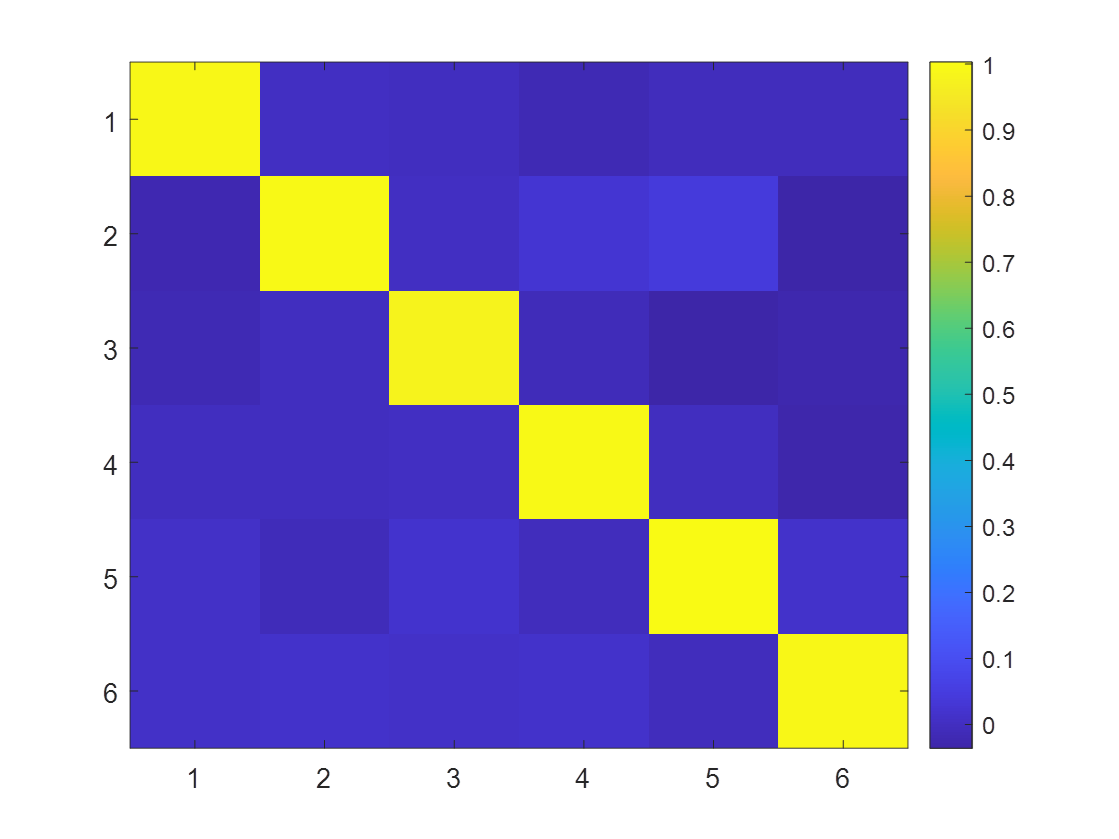
\includegraphics[width=0.55\textwidth]{noA_blk_A.png}}%
	}
	\caption{LDS sample with labels}
	\label{fig:noA labeled}
\end{figure}

This time the mixing of loading (\(\mathbf{d}\) and \(\mathbf{C}\)) is not fine. That reminds me that \textbf{I may need to make loading within cluster related by MV-(Poisson)-GLM directly.}



\subsubsection{Unlabeled Data: Clustering}
Again, all results can be found in this \href{https://github.com/weigcdsb/state-space-clustering/tree/main/results/gif}{folder}. The code can be found in this \href{https://github.com/weigcdsb/state-space-clustering/tree/main/LDS/blkDiag}{folder}.

Besides fitting 3 clusters with 10 neurons each, I further fit a larger scale example (50 neurons for each cluster). 


\clearpage


\section{TODO}
\begin{enumerate}
	\def\labelenumi{(\arabic{enumi})}
	\item
	Think about MV-(Poisson)-GLM. Check \href{https://www.tandfonline.com/doi/full/10.1080/03610926.2012.743565?journalCode=lsta20}{ref1} and \href{https://www.tandfonline.com/doi/full/10.1080/02664763.2021.1877637?src=recsys}{ref2}.
	\item
	After resolving (1), see if the MCMC is still trapped in local optima sometimes. Now, the chain seems will get stuck in local mode. Maybe updating the loading as a whole will remedy the problem a bit.
	\item
	Find a more efficient way to generate new cluster parameters, otherwise the newly generated ones will always be rejected.
	\item
	improve DPMM. In current brute force implementation, the number of potential clusters can even go beyond number of neurons (\(N\)). There are several improvements, e.g. \href{https://link.springer.com/article/10.1007/s11222-009-9150-y}{Kalli et al., 2011}, \href{http://proceedings.mlr.press/v37/gea15.html}{Ge et al., 2015} and \href{https://link.springer.com/article/10.1007/s11222-014-9471-3}{Hastie et al, 2015}. Check them later.
	\item
	After all of them are resolved, switch to GP version
	
\end{enumerate}


\end{document}






